\input{header.tex}
\input{newcommands.tex}


\title{Illustrationen zu Sachaufgaben mit Ti\textit{k}Z zeichnen}
\author{Fortbildungsmaterial für MINT-Lehrkräfte}
\date{23. November 2026}
\pagestyle{plain}
\setlength{\parskip}{1.5em} % Abstand zwischen Absätzen (Handreichungen)
\setlength{\emergencystretch}{2em} % lange \texttt-Wörter umbrechen statt über den Rand


\begin{document}

\maketitle

Ein Springbrunnen, ein Freistoß, ein Lkw unter einem Torbogen: Sachaufgaben werden verständlicher, wenn eine kleine Skizze die Situation zeigt. Lehrbücher machen das auf jeder Seite. Mit Ti\textit{k}Z gelingen solche Bilder auch im eigenen Arbeitsblatt, und zwar maßstäblich, in Vektorqualität und jederzeit änderbar.

Diese Handreichung zeigt Schritt für Schritt, wie solche Illustrationen entstehen: erst der Maßstab, dann Untergründe, Figuren, Flugbahnen und Gegenstände, schließlich neun vollständige Beispiele. Am Ende steht, wie aus demselben Bild ein Lösungsbild mit Koordinatensystem wird und wie Emoji-Köpfe mit Sprechblasen eine Fehlersuche tragen.

\begin{hinweis}[Drei Leitlinien]
\begin{itemize}
	\item \textbf{In Metern zeichnen.} Der Maßstab steht einmal in den Optionen der \texttt{tikzpicture}. Danach sind alle Koordinaten die Zahlen aus der Aufgabe.
	\item \textbf{Nur zeigen, was gegeben ist.} Die Skizze verrät keine Ergebnisse. Scheitelpunkt, Nullstellen und Rechenwege gehören ins Lösungsbild.
	\item \textbf{Sparsam beschriften.} Zwei oder drei dezente Maßangaben genügen. Der Rest steht im Aufgabentext.
\end{itemize}
\end{hinweis}



%%%%  KAPITEL  %%%%
\section{Zutaten}

Alle Beispiele kommen mit Ti\textit{k}Z und dem Paket \texttt{twemojis} für die Figuren aus. In der universalen \texttt{header.tex} ist beides geladen, ebenso die Bibliotheken \texttt{calc} und \texttt{shapes.callouts}. In einem eigenständigen Dokument gehören diese Zeilen in die Präambel:

\begin{lstlisting}[style=latex]
\usepackage{tikz}
\usetikzlibrary{calc, shapes.callouts, shadows}
\usepackage{twemojis}      % farbige Emojis, funktioniert mit pdflatex
\end{lstlisting}

Die universale \texttt{newcommands.tex} stellt außerdem fünf kleine Befehle bereit, die in dieser Handreichung immer wieder vorkommen:

\begin{itemize}
	\item \texttt{\textbackslash emojifigur}\texttt{[Optionen]\{(x,y)\}\{Name\}\{Höhe\}}\\ Ein Emoji steht auf dem Punkt \texttt{(x,y)} und ist so hoch wie angegeben.
	\item \texttt{\textbackslash masslinie}\texttt{\{(x1,y1)\}\{(x2,y2)\}\{Text\}}\\ Dezente Maßlinie mit Beschriftung in der Mitte.
	\item \texttt{\textbackslash skizzenraster}\texttt{\{xmin\}\{xmax\}\{ymin\}\{ymax\}\{Schritt\}\{x-Liste\}\{y-Liste\}}\\ Koordinatensystem, das hinter dem Bild liegt.
	\item \texttt{\textbackslash skizzenpunkt}\texttt{\{(x,y)\}\{Lage\}\{Text\}}\\ Markanter Punkt mit Beschriftung im Lösungsbild.
	\item \texttt{\textbackslash emojisprecher}\texttt{[Breite]\{x\}\{Emoji\}\{Name\}\{Aussage\}}\\ Emoji-Kopf mit Name und Sprechblase.
\end{itemize}

Dazu kommt der Schalter \texttt{\textbackslash ifmitKS}, mit dem ein Bild in zwei Fassungen entsteht (Kapitel~\ref{sec:loesungsbild}).



%%%%  KAPITEL  %%%%
\section{Das Grundprinzip: in Metern zeichnen}


%%%%  UNTERKAPITEL  %%%%
\subsection{Der Maßstab steht in den Optionen}

Mit \texttt{x=0.5cm, y=0.5cm} entspricht eine Längeneinheit im Bild einem halben Zentimeter auf dem Papier. Wer festlegt \enquote{eine Einheit ist ein Meter}, zeichnet ab jetzt mit den Zahlen aus der Aufgabe: Ein Mast in $\unit[10]{m}$ Entfernung steht bei $x=10$, eine $\unit[1{,}80]{m}$ große Person ist $1{,}8\cdot\unit[0{,}5]{cm}=\unit[0{,}9]{cm}$ hoch.

\begin{lstlisting}[style=latex]
\begin{tikzpicture}[x=0.5cm, y=0.5cm]   % 1 m entspricht 0,5 cm
	\draw[thick] (-1,0) -- (11,0);                   % Boden
	\draw[very thick, akzentblau] (10,0) -- (10,3);  % 3 m hoher Mast in 10 m Entfernung
	\emojifigur{(0,0)}{person standing}{0.9cm}       % 1,80 m groß
	\masslinie{(0,-0.8)}{(10,-0.8)}{$\unit[10]{m}$}
\end{tikzpicture}
\end{lstlisting}

\begin{ausgabe}
\centering
	\begin{tikzpicture}[x=0.5cm, y=0.5cm]   % 1 m entspricht 0,5 cm
		\draw[thick] (-1,0) -- (11,0);                   % Boden
		\draw[very thick, akzentblau] (10,0) -- (10,3);  % 3 m hoher Mast in 10 m Entfernung
		\emojifigur{(0,0)}{person standing}{0.9cm}       % 1,80 m groß
		\masslinie{(0,-0.8)}{(10,-0.8)}{$\unit[10]{m}$}
	\end{tikzpicture}
\end{ausgabe}

Der Maßstab richtet sich nach der Breite, die das Bild auf dem Blatt haben darf. Neben einem Aufgabentext sind das meist $5$ bis $7\,$cm, über die volle Breite bis zu $14\,$cm:

\begin{tabular}{@{}lll@{}}
	\toprule
	Ausdehnung der Situation & Maßstab & Bildbreite\\
	\midrule
	$\unit[10]{m}$ (Springbrunnen, Kugelstoß) & \texttt{x=0.5cm, y=0.5cm} & $5\,$cm\\
	$\unit[20]{m}$ (Freistoß), volle Breite & \texttt{x=0.6cm, y=0.6cm} & $12\,$cm\\
	$\unit[20]{m}$ (Brückenbogen), neben dem Text & \texttt{x=0.28cm, y=0.28cm} & $5{,}6\,$cm\\
	$\unit[100]{m}$ (Hängebrücke) & \texttt{x=0.05cm, y=0.05cm} & $5\,$cm\\
	\bottomrule
\end{tabular}

Beide Achsen bekommen denselben Maßstab. Nur so stimmen Höhen und Breiten im Bild zueinander, und nur so lässt sich später ein Koordinatensystem darunterlegen.


%%%%  UNTERKAPITEL  %%%%
\subsection{Die Reihenfolge der Ebenen}

Ti\textit{k}Z zeichnet in der Reihenfolge des Quelltexts, Späteres verdeckt Früheres. Für Sachskizzen hat sich diese Reihenfolge bewährt:

\begin{enumerate}
	\item Hintergrund und Untergrund (Wiese, Wasser, Mauer),
	\item Gegenstände und Figuren,
	\item die Kurve, um die es geht (Flugbahn, Seil, Bogen),
	\item Beschriftungen und Maßlinien.
\end{enumerate}



%%%%  KAPITEL  %%%%
\section{Untergründe und Hintergründe}


%%%%  UNTERKAPITEL  %%%%
\subsection{Wiese, Sand und Straße}

Ein Untergrund besteht aus einem flachen gefüllten Rechteck unter der Nulllinie und einer kräftigen Linie auf Höhe $y=0$. Die Farbe sagt, wo die Szene spielt.

\begin{lstlisting}[style=latex]

\begin{tikzpicture}[x=0.5cm, y=0.5cm]
	% Wiese
	\fill[green!25] (0,-0.5) rectangle (6,0);
	\draw[thick, green!40!black] (0,0) -- (6,0);
	% Sand
	\fill[orange!25] (7,-0.5) rectangle (13,0);
	\draw[thick, orange!50!black] (7,0) -- (13,0);
	% Straße
	\fill[gray!60] (14,-0.5) rectangle (20,0);
	\draw[white, dashed, thick] (14,-0.25) -- (20,-0.25);
	\draw[thick] (14,0) -- (20,0);
\end{tikzpicture}
\end{lstlisting}

\begin{ausgabe}
\centering
	
\begin{tikzpicture}[x=0.5cm, y=0.5cm]
		% Wiese
		\fill[green!25] (0,-0.5) rectangle (6,0);
		\draw[thick, green!40!black] (0,0) -- (6,0);
		% Sand
		\fill[orange!25] (7,-0.5) rectangle (13,0);
		\draw[thick, orange!50!black] (7,0) -- (13,0);
		% Straße
		\fill[gray!60] (14,-0.5) rectangle (20,0);
		\draw[white, dashed, thick] (14,-0.25) -- (20,-0.25);
		\draw[thick] (14,0) -- (20,0);
	\end{tikzpicture}
\end{ausgabe}


%%%%  UNTERKAPITEL  %%%%
\subsection{Wasser mit Wellen}

Wasser ist eine hellblaue Fläche mit einer dunkleren Oberkante. Kleine Bögen aus einer \texttt{\textbackslash foreach}-Schleife deuten Wellen an. Liegt das Wasser \emph{vor} einem Gegenstand (Schiffsrumpf, Brückenpfeiler), wird es zuletzt und halb durchsichtig gezeichnet: \texttt{opacity=0.75}.

\begin{lstlisting}[style=latex]

\begin{tikzpicture}[x=0.5cm, y=0.5cm]
	\emojifigur{(6,-0.35)}{sailboat}{1.3cm}
	\fill[blue!30, opacity=0.75] (0,-1.2) rectangle (12,0);
	\draw[blue!60!black] (0,0) -- (12,0);
	\foreach \w in {0.5,2,...,11}
		\draw[blue!60, thin] (\w,-0.6) .. controls +(0.25,0.2) and +(-0.25,0.2) .. +(0.8,0);
\end{tikzpicture}
\end{lstlisting}

\begin{ausgabe}
\centering
	
\begin{tikzpicture}[x=0.5cm, y=0.5cm]
		\emojifigur{(6,-0.35)}{sailboat}{1.3cm}
		\fill[blue!30, opacity=0.75] (0,-1.2) rectangle (12,0);
		\draw[blue!60!black] (0,0) -- (12,0);
		\foreach \w in {0.5,2,...,11}
			\draw[blue!60, thin] (\w,-0.6) .. controls +(0.25,0.2) and +(-0.25,0.2) .. +(0.8,0);
	\end{tikzpicture}
\end{ausgabe}


%%%%  UNTERKAPITEL  %%%%
\subsection{Mauerwerk mit einer Öffnung}

Eine Mauer mit Durchfahrt entsteht aus einem Rechteck, aus dem die Öffnung ausgespart wird. Dafür sorgt \texttt{even odd rule}: Was von zwei Teilpfaden überdeckt wird, bleibt frei. Die Fugen sind waagerechte Linien und versetzte kurze senkrechte Striche. Ein \texttt{\textbackslash clip} mit demselben Pfad hält sie aus der Öffnung heraus.

\begin{lstlisting}[style=latex]
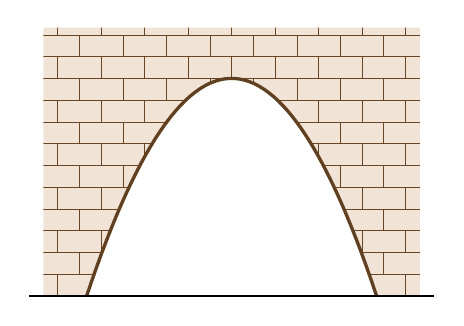
\begin{tikzpicture}[x=0.46cm, y=0.46cm]
	% Mauer mit parabelförmiger Öffnung (8 m breit, 6 m hoch)
	\fill[brown!22, even odd rule] (-5.2,0) rectangle (5.2,7.4)
		(-4,0) -- plot[domain=-4:4, samples=60] (\x,{-0.375*\x*\x+6}) -- cycle;
	% Fugen, auf die Mauerfläche beschränkt
	\begin{scope}[even odd rule]
		\clip (-5.2,0) rectangle (5.2,7.4)
			(-4,0) -- plot[domain=-4:4, samples=60] (\x,{-0.375*\x*\x+6}) -- cycle;
		\foreach \r in {0,...,12} {
			\draw[brown!55!black, very thin] (-5.2,\r*0.6) -- (5.2,\r*0.6);
			\foreach \c in {-5,...,5}
				\draw[brown!55!black, very thin] ({\c*1.2+0.6*mod(\r,2)},\r*0.6) -- ++(0,0.6);
		}
	\end{scope}
	\draw[very thick, brown!50!black, domain=-4:4, samples=60] plot (\x,{-0.375*\x*\x+6});
	\draw[thick] (-5.6,0) -- (5.6,0);
\end{tikzpicture}
\end{lstlisting}

\begin{ausgabe}
\centering
	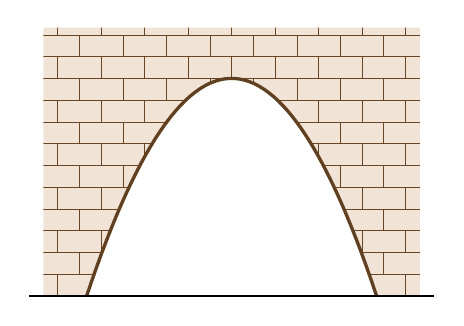
\begin{tikzpicture}[x=0.46cm, y=0.46cm]
		% Mauer mit parabelförmiger Öffnung (8 m breit, 6 m hoch)
		\fill[brown!22, even odd rule] (-5.2,0) rectangle (5.2,7.4)
			(-4,0) -- plot[domain=-4:4, samples=60] (\x,{-0.375*\x*\x+6}) -- cycle;
		% Fugen, auf die Mauerfläche beschränkt
		\begin{scope}[even odd rule]
			\clip (-5.2,0) rectangle (5.2,7.4)
				(-4,0) -- plot[domain=-4:4, samples=60] (\x,{-0.375*\x*\x+6}) -- cycle;
			\foreach \r in {0,...,12} {
				\draw[brown!55!black, very thin] (-5.2,\r*0.6) -- (5.2,\r*0.6);
				\foreach \c in {-5,...,5}
					\draw[brown!55!black, very thin] ({\c*1.2+0.6*mod(\r,2)},\r*0.6) -- ++(0,0.6);
			}
		\end{scope}
		\draw[very thick, brown!50!black, domain=-4:4, samples=60] plot (\x,{-0.375*\x*\x+6});
		\draw[thick] (-5.6,0) -- (5.6,0);
	\end{tikzpicture}
\end{ausgabe}

\begin{hinweis}[Muster lieber von Hand]
Die Ti\textit{k}Z-Muster \texttt{pattern=bricks} und \texttt{pattern=crosshatch} zeigt nicht jeder PDF-Betrachter an. Fugen und Netze aus einer Schleife sind in jedem Betrachter und im Druck zu sehen.
\end{hinweis}



%%%%  KAPITEL  %%%%
\section{Figuren mit Emojis}


%%%%  UNTERKAPITEL  %%%%
\subsection{Emojis im Text und im Bild}

Das Paket \texttt{twemojis} bringt die Emojis, die man vom Handy kennt, als Vektorgrafik mit. \texttt{\textbackslash texttwemoji\{Name\}} setzt ein Emoji in Schriftgröße in den Text, \texttt{\textbackslash twemoji[height=...]\{Name\}} in beliebiger Größe. Die Namen sind die englischen Unicode-Namen in Kleinbuchstaben.

\begin{lstlisting}[style=latex]
\texttwemoji{light bulb} Tipp: Zeichne zuerst den Scheitelpunkt ein. \qquad
\twemoji[height=8mm]{soccer ball} \twemoji[height=8mm]{stopwatch} \twemoji[height=8mm]{thinking face}
\end{lstlisting}

\begin{ausgabe}
\centering
	\texttwemoji{light bulb} Tipp: Zeichne zuerst den Scheitelpunkt ein. \qquad
	\twemoji[height=8mm]{soccer ball} \twemoji[height=8mm]{stopwatch} \twemoji[height=8mm]{thinking face}
\end{ausgabe}

In einer Skizze soll die Figur auf dem Boden stehen und die richtige Größe haben. Das erledigt \texttt{\textbackslash emojifigur}: Der Punkt ist die Stelle, an der die Füße stehen, die Höhe ergibt sich aus Körpergröße mal Maßstab. Mit \texttt{xscale=-1} im optionalen Argument schaut die Figur in die andere Richtung.

\begin{lstlisting}[style=latex]
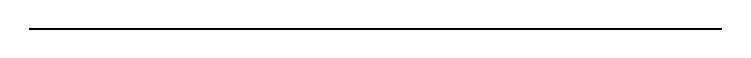
\begin{tikzpicture}[x=1cm, y=1cm]   % 1 m entspricht 1 cm
	\draw[thick] (-0.5,0) -- (8.3,0);
	\emojifigur{(0.5,0)}{man standing}{1.8cm}
	\emojifigur{(1.8,0)}{woman standing}{1.7cm}
	\emojifigur{(3.1,0)}{person standing}{1.2cm}
	\emojifigur{(5,0)}{deciduous tree}{3cm}
	\emojifigur[xscale=-1]{(7.3,0)}{person running}{1.8cm}
\end{tikzpicture}
\end{lstlisting}

\begin{ausgabe}
\centering
	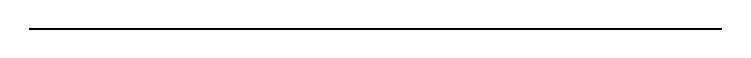
\begin{tikzpicture}[x=1cm, y=1cm]   % 1 m entspricht 1 cm
		\draw[thick] (-0.5,0) -- (8.3,0);
		\emojifigur{(0.5,0)}{man standing}{1.8cm}
		\emojifigur{(1.8,0)}{woman standing}{1.7cm}
		\emojifigur{(3.1,0)}{person standing}{1.2cm}
		\emojifigur{(5,0)}{deciduous tree}{3cm}
		\emojifigur[xscale=-1]{(7.3,0)}{person running}{1.8cm}
	\end{tikzpicture}
\end{ausgabe}


%%%%  UNTERKAPITEL  %%%%
\subsection{Nützliche Emojis für Sachaufgaben}

Die folgende Auswahl deckt die meisten Sachaufgaben der Sekundarstufe ab. Die vollständige Liste steht in der Dokumentation des Pakets (\texttt{texdoc twemojis}).

\begin{lstlisting}[style=latex]
\twemoji[height=6mm]{man standing}  \twemoji[height=6mm]{soccer ball}  \twemoji[height=6mm]{house}
\end{lstlisting}

\begin{ausgabe}
\small
\textbf{Stehende und bewegte Personen}\\[1mm]
\begin{tabular}{@{}clclcl@{}}
\twemoji[height=6mm]{man standing} & \texttt{man standing} & \twemoji[height=6mm]{woman standing} & \texttt{woman standing} & \twemoji[height=6mm]{person standing} & \texttt{person standing}\\[0.5mm]
\twemoji[height=6mm]{person walking} & \texttt{person walking} & \twemoji[height=6mm]{person running} & \texttt{person running} & \twemoji[height=6mm]{person biking} & \texttt{person biking}\\[0.5mm]
\twemoji[height=6mm]{person swimming} & \texttt{person swimming} & \twemoji[height=6mm]{person surfing} & \texttt{person surfing} & \twemoji[height=6mm]{person playing handball} & \texttt{person playing handball}\\[0.5mm]
\twemoji[height=6mm]{person bouncing ball} & \texttt{person bouncing ball} & \twemoji[height=6mm]{person cartwheeling} & \texttt{person cartwheeling} & \twemoji[height=6mm]{person climbing} & \texttt{person climbing}\\[0.5mm]
\end{tabular}\par\medskip
\textbf{Köpfe für Dialoge}\\[1mm]
\begin{tabular}{@{}clclcl@{}}
\twemoji[height=6mm]{boy} & \texttt{boy} & \twemoji[height=6mm]{girl} & \texttt{girl} & \twemoji[height=6mm]{child} & \texttt{child}\\[0.5mm]
\twemoji[height=6mm]{man} & \texttt{man} & \twemoji[height=6mm]{woman} & \texttt{woman} & \twemoji[height=6mm]{person} & \texttt{person}\\[0.5mm]
\twemoji[height=6mm]{man teacher} & \texttt{man teacher} & \twemoji[height=6mm]{woman teacher} & \texttt{woman teacher} & \twemoji[height=6mm]{thinking face} & \texttt{thinking face}\\[0.5mm]
\end{tabular}\par\medskip
\textbf{Sport und Spiel}\\[1mm]
\begin{tabular}{@{}clclcl@{}}
\twemoji[height=6mm]{soccer ball} & \texttt{soccer ball} & \twemoji[height=6mm]{basketball} & \texttt{basketball} & \twemoji[height=6mm]{volleyball} & \texttt{volleyball}\\[0.5mm]
\twemoji[height=6mm]{tennis} & \texttt{tennis} & \twemoji[height=6mm]{goal net} & \texttt{goal net} & \twemoji[height=6mm]{skateboard} & \texttt{skateboard}\\[0.5mm]
\twemoji[height=6mm]{kite} & \texttt{kite} & \twemoji[height=6mm]{balloon} & \texttt{balloon} & \twemoji[height=6mm]{stopwatch} & \texttt{stopwatch}\\[0.5mm]
\end{tabular}\par\medskip
\textbf{Fahrzeuge}\\[1mm]
\begin{tabular}{@{}clclcl@{}}
\twemoji[height=6mm]{automobile} & \texttt{automobile} & \twemoji[height=6mm]{delivery truck} & \texttt{delivery truck} & \twemoji[height=6mm]{bus} & \texttt{bus}\\[0.5mm]
\twemoji[height=6mm]{bicycle} & \texttt{bicycle} & \twemoji[height=6mm]{ship} & \texttt{ship} & \twemoji[height=6mm]{sailboat} & \texttt{sailboat}\\[0.5mm]
\twemoji[height=6mm]{airplane} & \texttt{airplane} & \twemoji[height=6mm]{rocket} & \texttt{rocket} & \twemoji[height=6mm]{tractor} & \texttt{tractor}\\[0.5mm]
\end{tabular}\par\medskip
\textbf{Gebäude, Natur und Dinge}\\[1mm]
\begin{tabular}{@{}clclcl@{}}
\twemoji[height=6mm]{house} & \texttt{house} & \twemoji[height=6mm]{deciduous tree} & \texttt{deciduous tree} & \twemoji[height=6mm]{evergreen tree} & \texttt{evergreen tree}\\[0.5mm]
\twemoji[height=6mm]{sun} & \texttt{sun} & \twemoji[height=6mm]{fountain} & \texttt{fountain} & \twemoji[height=6mm]{ladder} & \texttt{ladder}\\[0.5mm]
\twemoji[height=6mm]{light bulb} & \texttt{light bulb} & \twemoji[height=6mm]{money bag} & \texttt{money bag} & \twemoji[height=6mm]{bridge at night} & \texttt{bridge at night}\\[0.5mm]
\end{tabular}\par\medskip
\end{ausgabe}


%%%%  UNTERKAPITEL  %%%%
\subsection{Vielfalt: Hauttöne}

Personen-Emojis gibt es in fünf Hauttönen. Der Ton wird mit einem Doppelpunkt an den Namen gehängt. Bei mehreren Personen im Bild lohnt es sich, bewusst zu mischen.

\begin{lstlisting}[style=latex]
\twemoji[height=1cm]{girl}
\twemoji[height=1cm]{girl: light skin tone}
\twemoji[height=1cm]{girl: medium-light skin tone}
\twemoji[height=1cm]{girl: medium skin tone}
\twemoji[height=1cm]{girl: medium-dark skin tone}
\twemoji[height=1cm]{girl: dark skin tone}
\qquad
\twemoji[height=1cm]{man standing: medium skin tone}
\twemoji[height=1cm]{woman standing: dark skin tone}
\end{lstlisting}

\begin{ausgabe}
\centering
	\twemoji[height=1cm]{girl}
	\twemoji[height=1cm]{girl: light skin tone}
	\twemoji[height=1cm]{girl: medium-light skin tone}
	\twemoji[height=1cm]{girl: medium skin tone}
	\twemoji[height=1cm]{girl: medium-dark skin tone}
	\twemoji[height=1cm]{girl: dark skin tone}
	\qquad
	\twemoji[height=1cm]{man standing: medium skin tone}
	\twemoji[height=1cm]{woman standing: dark skin tone}
\end{ausgabe}


%%%%  UNTERKAPITEL  %%%%
\subsection{Alternativen: Piktogramm und tikzpeople}

Für den Schwarz-Weiß-Druck oder ohne das Paket \texttt{twemojis} genügt ein Piktogramm aus wenigen Strichen. Es wird in einer \texttt{scope} gezeichnet, die an die richtige Stelle verschoben und auf die Körpergröße skaliert ist. Die Figuren des Pakets \texttt{tikzpeople} (rechts) sind Büsten ohne Beine. Sie eignen sich für Dialoge, aber nicht für maßstäbliche Skizzen.

\begin{lstlisting}[style=latex]
\begin{tikzpicture}[x=1cm, y=1cm]
	\draw[thick] (-0.5,0) -- (5,0);
	% Piktogramm: steht bei x = 1 und ist 1,80 m groß
	\begin{scope}[shift={(1,0)}, scale=1.8]
		\draw[line width=1.6pt, line cap=round, line join=round]
			(-0.09,0) -- (-0.05,0.46) -- (0.05,0.46) -- (0.09,0);       % Beine
		\draw[line width=1.4pt, line cap=round]
			(-0.11,0.74) -- (-0.17,0.47) (0.11,0.74) -- (0.17,0.47);   % Arme
		\fill[rounded corners=1pt] (-0.11,0.44) rectangle (0.11,0.78); % Rumpf
		\fill (0,0.9) circle (0.095);                                  % Kopf
	\end{scope}
	% tikzpeople: Büste
	\node[alice, minimum size=1.8cm, anchor=south] at (3.5,0) {};
\end{tikzpicture}
\end{lstlisting}

\begin{ausgabe}
\centering
	\begin{tikzpicture}[x=1cm, y=1cm]
		\draw[thick] (-0.5,0) -- (5,0);
		% Piktogramm: steht bei x = 1 und ist 1,80 m groß
		\begin{scope}[shift={(1,0)}, scale=1.8]
			\draw[line width=1.6pt, line cap=round, line join=round]
				(-0.09,0) -- (-0.05,0.46) -- (0.05,0.46) -- (0.09,0);       % Beine
			\draw[line width=1.4pt, line cap=round]
				(-0.11,0.74) -- (-0.17,0.47) (0.11,0.74) -- (0.17,0.47);   % Arme
			\fill[rounded corners=1pt] (-0.11,0.44) rectangle (0.11,0.78); % Rumpf
			\fill (0,0.9) circle (0.095);                                  % Kopf
		\end{scope}
		% tikzpeople: Büste
		\node[alice, minimum size=1.8cm, anchor=south] at (3.5,0) {};
	\end{tikzpicture}
\end{ausgabe}



%%%%  KAPITEL  %%%%
\section{Flugbahnen und andere Kurven}


%%%%  UNTERKAPITEL  %%%%
\subsection{Eine Flugbahn mit Ball}

Die Kurve wird mit \texttt{plot} aus der Funktionsgleichung gezeichnet, gestrichelt und in zurückhaltendem Grau. Den Ball setzt man an zwei oder drei Stellen auf die Bahn. Die Höhe rechnet Ti\textit{k}Z selbst aus, wenn die Funktionsgleichung in der $y$-Koordinate steht. Wichtig sind die Klammern um \texttt{\textbackslash x-4}: Ohne sie rechnet pgf bei negativen Werten falsch.

\begin{lstlisting}[style=latex]
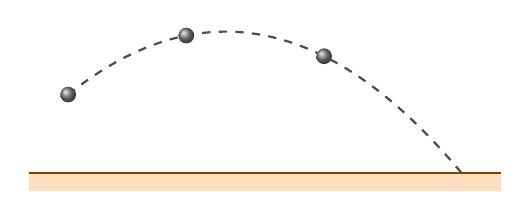
\begin{tikzpicture}[x=0.5cm, y=0.5cm]
	\fill[orange!25] (-1,-0.45) rectangle (11,0);
	\draw[thick, orange!50!black] (-1,0) -- (11,0);
	% Flugbahn h(x) = -0,1 (x-4)^2 + 3,6
	\draw[dashed, thick, gray!60!black, domain=0:10, samples=100]
		plot (\x,{-0.1*(\x-4)^2+3.6});
	% Kugel an drei Stellen der Bahn
	\foreach \b in {0,3,6.5}
		\shade[ball color=gray] (\b,{-0.1*(\b-4)^2+3.6}) circle (0.2);
\end{tikzpicture}
\end{lstlisting}

\begin{ausgabe}
\centering
	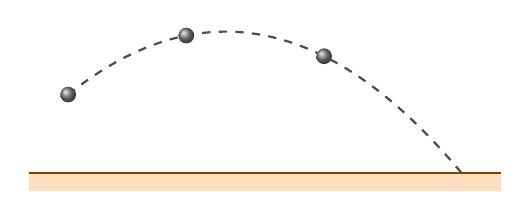
\begin{tikzpicture}[x=0.5cm, y=0.5cm]
		\fill[orange!25] (-1,-0.45) rectangle (11,0);
		\draw[thick, orange!50!black] (-1,0) -- (11,0);
		% Flugbahn h(x) = -0,1 (x-4)^2 + 3,6
		\draw[dashed, thick, gray!60!black, domain=0:10, samples=100]
			plot (\x,{-0.1*(\x-4)^2+3.6});
		% Kugel an drei Stellen der Bahn
		\foreach \b in {0,3,6.5}
			\shade[ball color=gray] (\b,{-0.1*(\b-4)^2+3.6}) circle (0.2);
	\end{tikzpicture}
\end{ausgabe}


%%%%  UNTERKAPITEL  %%%%
\subsection{Ein Wasserstrahl}

Wasser wirkt plastischer, wenn dieselbe Kurve zweimal übereinander liegt: unten breit und hell, darüber schmal und kräftig. Ein paar kurze Striche am Auftreffpunkt deuten Spritzer an.

\begin{lstlisting}[style=latex]
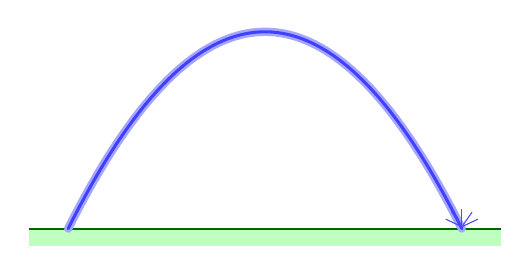
\begin{tikzpicture}[x=0.5cm, y=0.5cm]
	\fill[green!25] (-1,-0.45) rectangle (11,0);
	\draw[thick, green!40!black] (-1,0) -- (11,0);
	\draw[blue!35, line width=3pt, line cap=round, domain=0:10, samples=100]
		plot (\x,{-0.2*(\x-5)^2+5});
	\draw[blue!75, line width=1.1pt, line cap=round, domain=0:10, samples=100]
		plot (\x,{-0.2*(\x-5)^2+5});
	\foreach \a in {25,55,90,125,155} \draw[blue!70, thin] (10,0.05) -- ++(\a:0.45);
\end{tikzpicture}
\end{lstlisting}

\begin{ausgabe}
\centering
	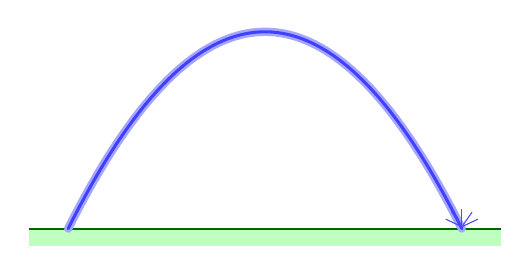
\begin{tikzpicture}[x=0.5cm, y=0.5cm]
		\fill[green!25] (-1,-0.45) rectangle (11,0);
		\draw[thick, green!40!black] (-1,0) -- (11,0);
		\draw[blue!35, line width=3pt, line cap=round, domain=0:10, samples=100]
			plot (\x,{-0.2*(\x-5)^2+5});
		\draw[blue!75, line width=1.1pt, line cap=round, domain=0:10, samples=100]
			plot (\x,{-0.2*(\x-5)^2+5});
		\foreach \a in {25,55,90,125,155} \draw[blue!70, thin] (10,0.05) -- ++(\a:0.45);
	\end{tikzpicture}
\end{ausgabe}


%%%%  UNTERKAPITEL  %%%%
\subsection{Ein hängendes Seil mit Hängern}

Auch senkrechte Verbindungen lassen sich berechnen: Die Schleife zieht an jeder Stelle einen Strich von der Fahrbahn bis zur Kurve.

\begin{lstlisting}[style=latex]
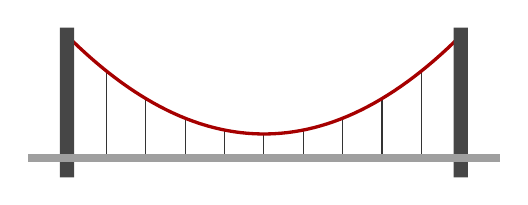
\begin{tikzpicture}[x=0.05cm, y=0.05cm]   % 1 m entspricht 0,05 cm
	\foreach \k in {10,20,...,90}
		\draw[thin, gray!40!black] (\k,0) -- (\k,{0.01*(\k-50)^2+5});
	\draw[very thick, red!65!black, domain=0:100, samples=60]
		plot (\x,{0.01*(\x-50)^2+5});
	\fill[gray!55!black] (-1.8,-6) rectangle (1.8,32) (98.2,-6) rectangle (101.8,32);
	\fill[gray!75] (-10,-2) rectangle (110,0);
\end{tikzpicture}
\end{lstlisting}

\begin{ausgabe}
\centering
	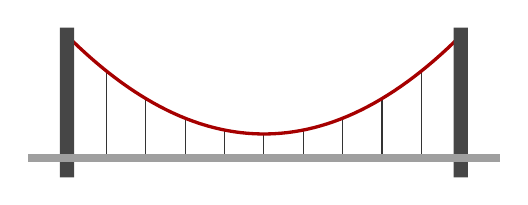
\begin{tikzpicture}[x=0.05cm, y=0.05cm]   % 1 m entspricht 0,05 cm
		\foreach \k in {10,20,...,90}
			\draw[thin, gray!40!black] (\k,0) -- (\k,{0.01*(\k-50)^2+5});
		\draw[very thick, red!65!black, domain=0:100, samples=60]
			plot (\x,{0.01*(\x-50)^2+5});
		\fill[gray!55!black] (-1.8,-6) rectangle (1.8,32) (98.2,-6) rectangle (101.8,32);
		\fill[gray!75] (-10,-2) rectangle (110,0);
	\end{tikzpicture}
\end{ausgabe}



%%%%  KAPITEL  %%%%
\section{Sparsam bemaßen}

Maßlinien sind die häufigste Ursache für überladene Skizzen. Drei Regeln helfen:

\begin{itemize}
	\item Höchstens zwei bis drei Maße pro Bild, und nur solche, die in der Aufgabe gegeben sind.
	\item Dünn und grau statt dick und rot. Die Maße sollen lesbar sein, aber nicht das Bild beherrschen.
	\item Liegen mehrere Entfernungen auf einer Linie, ersetzt eine Entfernungsleiste mehrere gestapelte Maßlinien.
\end{itemize}


%%%%  UNTERKAPITEL  %%%%
\subsection{Die Maßlinie}

\texttt{\textbackslash masslinie} zeichnet eine dünne graue Linie mit Endstrichen und setzt den Text auf weißem Grund in die Mitte. Sie liegt mit etwas Abstand neben dem Gegenstand. Gepunktete Hilfslinien zeigen, worauf sie sich bezieht.

\begin{lstlisting}[style=latex]
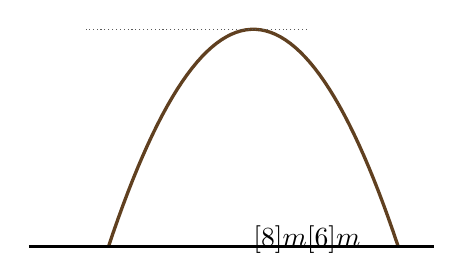
\begin{tikzpicture}[x=0.46cm, y=0.46cm]
	\draw[very thick, brown!50!black, domain=-4:4, samples=60] plot (\x,{-0.375*\x*\x+6});
	\draw[thick] (-6.2,0) -- (5,0);
	\masslinie{(-4,-0.8)}{(4,-0.8)}{$\unit[8]{m}$}
	\draw[thin, black!65, densely dotted] (0,6) -- (-6.1,6);
	\masslinie{(-5.8,0)}{(-5.8,6)}{$\unit[6]{m}$}
\end{tikzpicture}
\end{lstlisting}

\begin{ausgabe}
\centering
	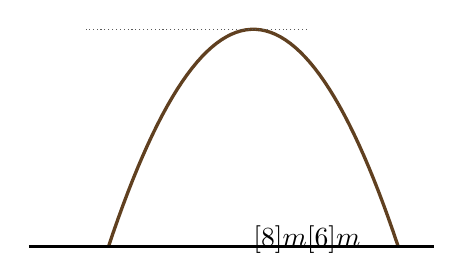
\begin{tikzpicture}[x=0.46cm, y=0.46cm]
		\draw[very thick, brown!50!black, domain=-4:4, samples=60] plot (\x,{-0.375*\x*\x+6});
		\draw[thick] (-6.2,0) -- (5,0);
		\masslinie{(-4,-0.8)}{(4,-0.8)}{$\unit[8]{m}$}
		\draw[thin, black!65, densely dotted] (0,6) -- (-6.1,6);
		\masslinie{(-5.8,0)}{(-5.8,6)}{$\unit[6]{m}$}
	\end{tikzpicture}
\end{ausgabe}


%%%%  UNTERKAPITEL  %%%%
\subsection{Die Entfernungsleiste}

Beim Freistoß liegen drei Entfernungen auf dem Boden: Mauer, höchster Punkt und Tor. Statt dreier Maßlinien untereinander genügt eine Leiste mit Strichen und Zahlen.

\begin{lstlisting}[style=latex]
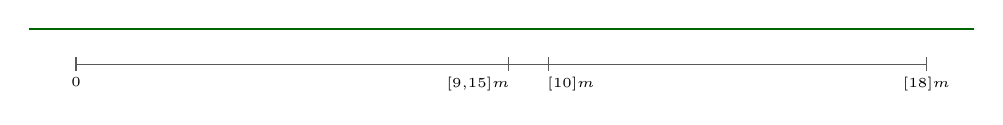
\begin{tikzpicture}[x=0.6cm, y=0.6cm]
	\draw[thick, green!40!black] (-1,0) -- (19,0);
	% Entfernungsleiste
	\draw[thin, black!65] (0,-0.75) -- (18,-0.75);
	\foreach \k in {0,9.15,10,18} \draw[thin, black!65] (\k,-0.6) -- (\k,-0.9);
	\node[font=\tiny, below, inner sep=2pt] at (0,-0.9) {$0$};
	\node[font=\tiny, below left, inner sep=2pt] at (9.3,-0.9) {$\unit[9{,}15]{m}$};
	\node[font=\tiny, below right, inner sep=2pt] at (9.85,-0.9) {$\unit[10]{m}$};
	\node[font=\tiny, below, inner sep=2pt] at (18,-0.9) {$\unit[18]{m}$};
\end{tikzpicture}
\end{lstlisting}

\begin{ausgabe}
\begin{passend}
	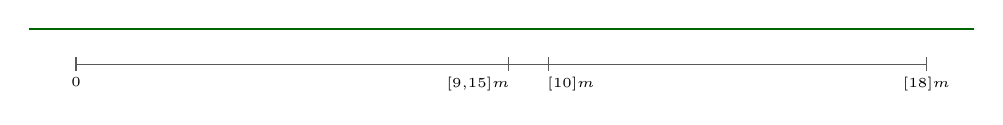
\begin{tikzpicture}[x=0.6cm, y=0.6cm]
		\draw[thick, green!40!black] (-1,0) -- (19,0);
		% Entfernungsleiste
		\draw[thin, black!65] (0,-0.75) -- (18,-0.75);
		\foreach \k in {0,9.15,10,18} \draw[thin, black!65] (\k,-0.6) -- (\k,-0.9);
		\node[font=\tiny, below, inner sep=2pt] at (0,-0.9) {$0$};
		\node[font=\tiny, below left, inner sep=2pt] at (9.3,-0.9) {$\unit[9{,}15]{m}$};
		\node[font=\tiny, below right, inner sep=2pt] at (9.85,-0.9) {$\unit[10]{m}$};
		\node[font=\tiny, below, inner sep=2pt] at (18,-0.9) {$\unit[18]{m}$};
	\end{tikzpicture}
\end{passend}
\end{ausgabe}


%%%%  UNTERKAPITEL  %%%%
\subsection{Variablen statt Zahlen}

Oft ist es hilfreicher, die Bedeutung der Variablen zu zeigen als eine Zahl: Was ist $x$, was ist $h(x)$? Eine gepunktete Senkrechte vom Boden zur Kurve und eine Maßlinie am Boden genügen.

\begin{lstlisting}[style=latex]
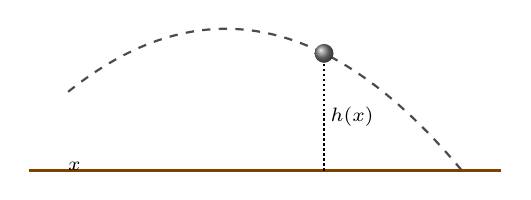
\begin{tikzpicture}[x=0.5cm, y=0.5cm]
	\draw[thick, orange!50!black] (-1,0) -- (11,0);
	\draw[dashed, thick, gray!60!black, domain=0:10, samples=100] plot (\x,{-0.1*(\x-4)^2+3.6});
	\shade[ball color=gray] (6.5,2.975) circle (0.24);
	\draw[densely dotted, thick] (6.5,0) -- (6.5,2.72)
		node[midway, right, font=\scriptsize, inner sep=2pt] {$h(x)$};
	\masslinie{(0,-1.1)}{(6.5,-1.1)}{\scriptsize $x$}
\end{tikzpicture}
\end{lstlisting}

\begin{ausgabe}
\centering
	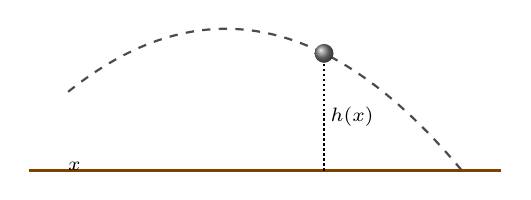
\begin{tikzpicture}[x=0.5cm, y=0.5cm]
		\draw[thick, orange!50!black] (-1,0) -- (11,0);
		\draw[dashed, thick, gray!60!black, domain=0:10, samples=100] plot (\x,{-0.1*(\x-4)^2+3.6});
		\shade[ball color=gray] (6.5,2.975) circle (0.24);
		\draw[densely dotted, thick] (6.5,0) -- (6.5,2.72)
			node[midway, right, font=\scriptsize, inner sep=2pt] {$h(x)$};
		\masslinie{(0,-1.1)}{(6.5,-1.1)}{\scriptsize $x$}
	\end{tikzpicture}
\end{ausgabe}



%%%%  KAPITEL  %%%%
\section{Gegenstände selbst zeichnen}

Emojis zeigen Fahrzeuge von der Seite. Für Aufgaben wie \enquote{Passt der Lkw durch den Torbogen?} braucht man die Ansicht von vorn, und zwar mit den Maßen aus der Aufgabe. Solche Gegenstände bestehen aus wenigen Rechtecken und Kreisen. Entscheidend ist der Umriss: Breite und Höhe stimmen exakt, alles andere ist Dekoration.


%%%%  UNTERKAPITEL  %%%%
\subsection{Ein Lkw von vorn}

\begin{lstlisting}[style=latex]
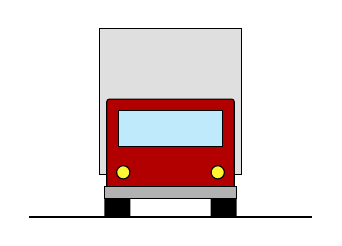
\begin{tikzpicture}[x=0.6cm, y=0.6cm]
	\draw[thick] (-3,0) -- (3,0);
	% Lkw: 3 m breit, 4 m hoch
	\fill[black] (-1.4,0) rectangle (-0.85,0.6) (0.85,0) rectangle (1.4,0.6);       % Räder
	\fill[gray!25, draw=black] (-1.5,0.9) rectangle (1.5,4);                         % Aufbau
	\fill[red!70!black, draw=black, rounded corners=1pt] (-1.35,0.45) rectangle (1.35,2.5); % Fahrerhaus
	\fill[cyan!25, draw=black] (-1.1,1.5) rectangle (1.1,2.25);                      % Scheibe
	\fill[gray!60, draw=black] (-1.4,0.4) rectangle (1.4,0.65);                      % Stoßstange
	\fill[yellow!80, draw=black] (-1,0.95) circle (0.14) (1,0.95) circle (0.14);     % Scheinwerfer
\end{tikzpicture}
\end{lstlisting}

\begin{ausgabe}
\centering
	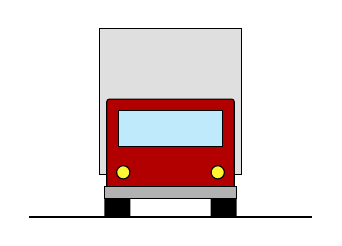
\begin{tikzpicture}[x=0.6cm, y=0.6cm]
		\draw[thick] (-3,0) -- (3,0);
		% Lkw: 3 m breit, 4 m hoch
		\fill[black] (-1.4,0) rectangle (-0.85,0.6) (0.85,0) rectangle (1.4,0.6);       % Räder
		\fill[gray!25, draw=black] (-1.5,0.9) rectangle (1.5,4);                         % Aufbau
		\fill[red!70!black, draw=black, rounded corners=1pt] (-1.35,0.45) rectangle (1.35,2.5); % Fahrerhaus
		\fill[cyan!25, draw=black] (-1.1,1.5) rectangle (1.1,2.25);                      % Scheibe
		\fill[gray!60, draw=black] (-1.4,0.4) rectangle (1.4,0.65);                      % Stoßstange
		\fill[yellow!80, draw=black] (-1,0.95) circle (0.14) (1,0.95) circle (0.14);     % Scheinwerfer
	\end{tikzpicture}
\end{ausgabe}


%%%%  UNTERKAPITEL  %%%%
\subsection{Ein Schiff von vorn}

Der Rumpf reicht unter die Wasserlinie, das Wasser wird danach halb durchsichtig darübergelegt. Über Wasser ist das Schiff genau $\unit[8]{m}$ breit und $\unit[4]{m}$ hoch.

\begin{lstlisting}[style=latex]
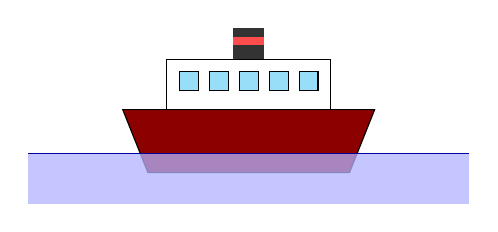
\begin{tikzpicture}[x=0.4cm, y=0.4cm]
	% Schiff: 8 m breit, ragt 4 m aus dem Wasser
	\fill[red!55!black, draw=black] (-4,1.4) -- (4,1.4) -- (3.2,-0.6) -- (-3.2,-0.6) -- cycle; % Rumpf
	\fill[white, draw=black] (-2.6,1.4) rectangle (2.6,3);                                     % Aufbau
	\foreach \f in {-1.9,-0.95,0,0.95,1.9}
		\fill[cyan!40, draw=black, thin] (\f-0.3,2.0) rectangle (\f+0.3,2.6);                  % Fenster
	\fill[black!80] (-0.5,3) rectangle (0.5,4);                                                % Schornstein
	\fill[red!70] (-0.5,3.45) rectangle (0.5,3.7);
	% Wasser davor
	\fill[blue!30, opacity=0.75] (-7,-1.6) rectangle (7,0);
	\draw[blue!60!black] (-7,0) -- (7,0);
\end{tikzpicture}
\end{lstlisting}

\begin{ausgabe}
\centering
	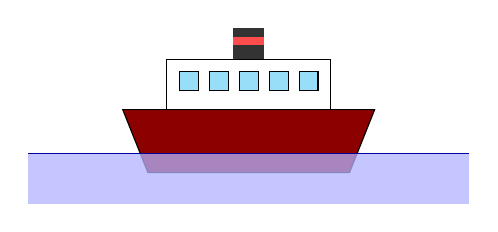
\begin{tikzpicture}[x=0.4cm, y=0.4cm]
		% Schiff: 8 m breit, ragt 4 m aus dem Wasser
		\fill[red!55!black, draw=black] (-4,1.4) -- (4,1.4) -- (3.2,-0.6) -- (-3.2,-0.6) -- cycle; % Rumpf
		\fill[white, draw=black] (-2.6,1.4) rectangle (2.6,3);                                     % Aufbau
		\foreach \f in {-1.9,-0.95,0,0.95,1.9}
			\fill[cyan!40, draw=black, thin] (\f-0.3,2.0) rectangle (\f+0.3,2.6);                  % Fenster
		\fill[black!80] (-0.5,3) rectangle (0.5,4);                                                % Schornstein
		\fill[red!70] (-0.5,3.45) rectangle (0.5,3.7);
		% Wasser davor
		\fill[blue!30, opacity=0.75] (-7,-1.6) rectangle (7,0);
		\draw[blue!60!black] (-7,0) -- (7,0);
	\end{tikzpicture}
\end{ausgabe}


%%%%  UNTERKAPITEL  %%%%
\subsection{Ein Tor in der Seitenansicht}

\begin{lstlisting}[style=latex]
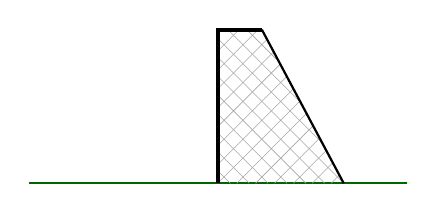
\begin{tikzpicture}[x=0.8cm, y=0.8cm]
	\draw[thick, green!40!black] (-3,0) -- (3,0);
	% Netz: Schleife, auf die Netzfläche beschränkt
	\begin{scope}
		\clip (0,0) -- (0,2.44) -- (0.7,2.44) -- (2,0) -- cycle;
		\foreach \n in {-3,-2.7,...,3}
			\draw[gray!70, very thin] (\n,0) -- ++(2.6,2.6) (2+\n,0) -- ++(-2.6,2.6);
	\end{scope}
	\draw[thick] (0.7,2.44) -- (2,0);
	\draw[line width=1.4pt] (0,0) -- (0,2.44) -- (0.7,2.44);   % Pfosten und Latte, 2,44 m hoch
	\emojifigur{(-1.5,0)}{soccer ball}{0.35cm}
\end{tikzpicture}
\end{lstlisting}

\begin{ausgabe}
\centering
	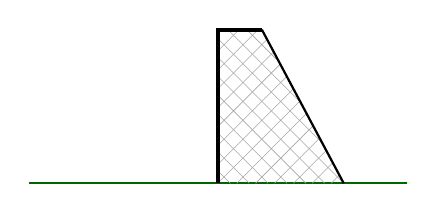
\begin{tikzpicture}[x=0.8cm, y=0.8cm]
		\draw[thick, green!40!black] (-3,0) -- (3,0);
		% Netz: Schleife, auf die Netzfläche beschränkt
		\begin{scope}
			\clip (0,0) -- (0,2.44) -- (0.7,2.44) -- (2,0) -- cycle;
			\foreach \n in {-3,-2.7,...,3}
				\draw[gray!70, very thin] (\n,0) -- ++(2.6,2.6) (2+\n,0) -- ++(-2.6,2.6);
		\end{scope}
		\draw[thick] (0.7,2.44) -- (2,0);
		\draw[line width=1.4pt] (0,0) -- (0,2.44) -- (0.7,2.44);   % Pfosten und Latte, 2,44 m hoch
		\emojifigur{(-1.5,0)}{soccer ball}{0.35cm}
	\end{tikzpicture}
\end{ausgabe}


%%%%  UNTERKAPITEL  %%%%
\subsection{Haus und Baum}

\begin{lstlisting}[style=latex]
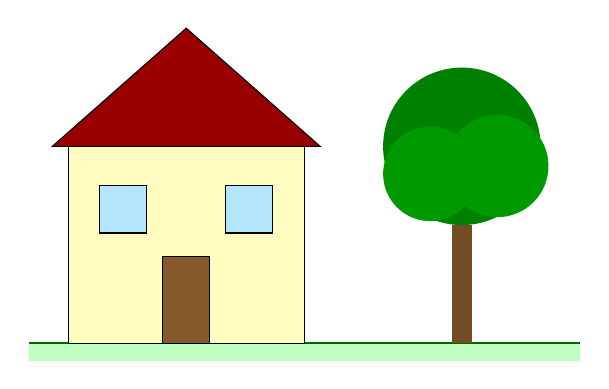
\begin{tikzpicture}[x=0.5cm, y=0.5cm]
	\fill[green!25] (-1,-0.45) rectangle (13,0);
	\draw[thick, green!40!black] (-1,0) -- (13,0);
	% Haus: 6 m breit, Traufe 5 m, First 8 m
	\fill[yellow!25, draw=black] (0,0) rectangle (6,5);
	\fill[red!60!black, draw=black] (-0.4,5) -- (3,8) -- (6.4,5) -- cycle;
	\fill[brown!70!black, draw=black] (2.4,0) rectangle (3.6,2.2);
	\fill[cyan!30, draw=black] (0.8,2.8) rectangle (2,4) (4,2.8) rectangle (5.2,4);
	% Baum: 7 m hoch
	\fill[brown!60!black] (9.75,0) rectangle (10.25,3);
	\fill[green!50!black] (10,5) circle (2);
	\fill[green!60!black] (9.2,4.3) circle (1.2) (10.9,4.5) circle (1.3);
\end{tikzpicture}
\end{lstlisting}

\begin{ausgabe}
\centering
	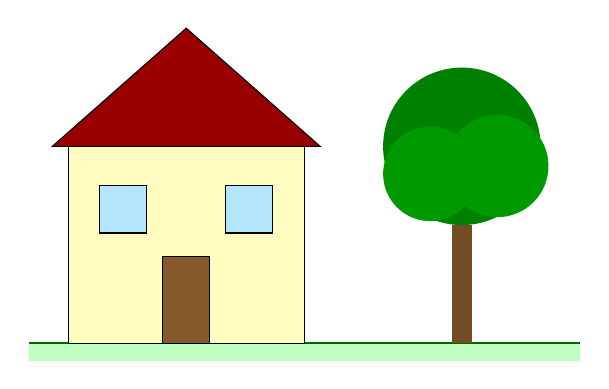
\begin{tikzpicture}[x=0.5cm, y=0.5cm]
		\fill[green!25] (-1,-0.45) rectangle (13,0);
		\draw[thick, green!40!black] (-1,0) -- (13,0);
		% Haus: 6 m breit, Traufe 5 m, First 8 m
		\fill[yellow!25, draw=black] (0,0) rectangle (6,5);
		\fill[red!60!black, draw=black] (-0.4,5) -- (3,8) -- (6.4,5) -- cycle;
		\fill[brown!70!black, draw=black] (2.4,0) rectangle (3.6,2.2);
		\fill[cyan!30, draw=black] (0.8,2.8) rectangle (2,4) (4,2.8) rectangle (5.2,4);
		% Baum: 7 m hoch
		\fill[brown!60!black] (9.75,0) rectangle (10.25,3);
		\fill[green!50!black] (10,5) circle (2);
		\fill[green!60!black] (9.2,4.3) circle (1.2) (10.9,4.5) circle (1.3);
	\end{tikzpicture}
\end{ausgabe}



%%%%  KAPITEL  %%%%
\section{Vollständige Beispiele}

Die folgenden neun Skizzen sind fertige Vorlagen. Die ersten sechs gehören zu quadratischen Funktionen, die letzten drei zeigen, dass dieselben Bausteine auch für den Satz des Pythagoras, den Strahlensatz und die Steigung taugen. Unter jeder Überschrift steht die Aufgabe, zu der das Bild passt.


%%%%  UNTERKAPITEL  %%%%
\subsection{Springbrunnen}

Der Wasserstrahl folgt $h(x)=-0{,}2(x-5)^2+5$. Ein $\unit[1{,}80]{m}$ großer Mann steht $\unit[8{,}5]{m}$ von der Düse entfernt. Geht der Strahl über seinen Kopf hinweg?

\begin{lstlisting}[style=latex]
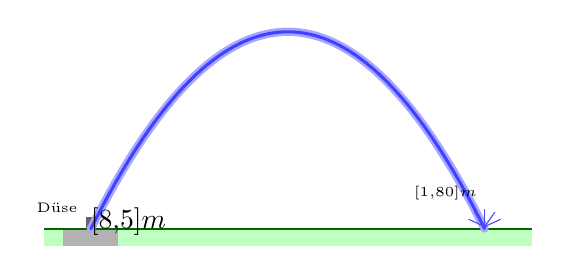
\begin{tikzpicture}[x=0.5cm, y=0.5cm]
	\fill[green!25] (-1.2,-0.45) rectangle (11.2,0); \fill[gray!60] (-0.7,-0.45) rectangle (0.7,0);
	\draw[thick, green!40!black] (-1.2,0) -- (11.2,0);
	\fill[gray!80!black] (-0.12,0) rectangle (0.12,0.3);
	\draw[blue!35, line width=3pt, line cap=round, domain=0:10, samples=100] plot (\x,{-0.2*(\x-5)^2+5});
	\draw[blue!75, line width=1.1pt, line cap=round, domain=0:10, samples=100] plot (\x,{-0.2*(\x-5)^2+5});
	\foreach \a in {25,55,90,125,155} \draw[blue!70, thin] (10,0.05) -- ++(\a:0.45);
	\emojifigur{(8.5,0)}{man standing}{0.9cm}
	\node[font=\tiny, above left] at (-0.1,0.15) {Düse};
	\masslinie{(0,-1.1)}{(8.5,-1.1)}{$\unit[8{,}5]{m}$}
	\node[font=\tiny, left, inner sep=2pt] at (8.05,0.9) {$\unit[1{,}80]{m}$};
\end{tikzpicture}
\end{lstlisting}

\begin{ausgabe}
\centering
	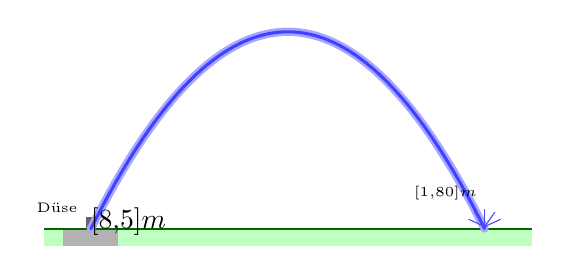
\begin{tikzpicture}[x=0.5cm, y=0.5cm]
		\fill[green!25] (-1.2,-0.45) rectangle (11.2,0); \fill[gray!60] (-0.7,-0.45) rectangle (0.7,0);
		\draw[thick, green!40!black] (-1.2,0) -- (11.2,0);
		\fill[gray!80!black] (-0.12,0) rectangle (0.12,0.3);
		\draw[blue!35, line width=3pt, line cap=round, domain=0:10, samples=100] plot (\x,{-0.2*(\x-5)^2+5});
		\draw[blue!75, line width=1.1pt, line cap=round, domain=0:10, samples=100] plot (\x,{-0.2*(\x-5)^2+5});
		\foreach \a in {25,55,90,125,155} \draw[blue!70, thin] (10,0.05) -- ++(\a:0.45);
		\emojifigur{(8.5,0)}{man standing}{0.9cm}
		\node[font=\tiny, above left] at (-0.1,0.15) {Düse};
		\masslinie{(0,-1.1)}{(8.5,-1.1)}{$\unit[8{,}5]{m}$}
		\node[font=\tiny, left, inner sep=2pt] at (8.05,0.9) {$\unit[1{,}80]{m}$};
	\end{tikzpicture}
\end{ausgabe}


%%%%  UNTERKAPITEL  %%%%
\subsection{Kugelstoßen}

Die Kugel fliegt auf der Bahn $h(x)=-0{,}1(x-4)^2+3{,}6$. Gesucht sind Abstoßhöhe, größte Höhe und Stoßweite. Das Bild zeigt nur, was $x$ und $h(x)$ bedeuten.

\begin{lstlisting}[style=latex]
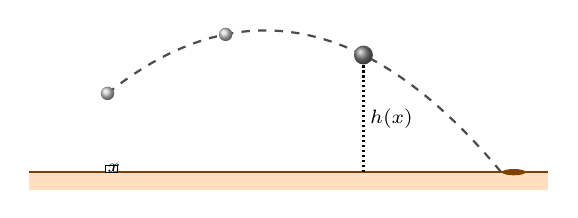
\begin{tikzpicture}[x=0.5cm, y=0.5cm]
	\fill[orange!25] (-2,-0.45) rectangle (11.2,0);
	\draw[thick, orange!50!black] (-2,0) -- (11.2,0);
	\fill[white, draw=black] (-0.05,0) rectangle (0.25,0.18);
	\emojifigur[xscale=-1]{(-0.85,0)}{person playing handball}{1.25cm}
	\draw[dashed, thick, gray!60!black, domain=0:10, samples=100] plot (\x,{-0.1*(\x-4)^2+3.6});
	\shade[ball color=gray!40] (0,2) circle (0.17);
	\shade[ball color=gray!40] (3,3.5) circle (0.17);
	\shade[ball color=gray] (6.5,2.975) circle (0.24);
	\draw[densely dotted, thick] (6.5,0) -- (6.5,2.72) node[midway, right, font=\scriptsize, inner sep=2pt] {$h(x)$};
	\masslinie{(0,-1.1)}{(6.5,-1.1)}{\scriptsize $x$}
	\fill[orange!50!black] (10,0) ellipse (0.3 and 0.08);
\end{tikzpicture}
\end{lstlisting}

\begin{ausgabe}
\centering
	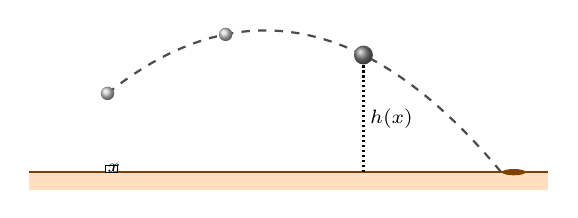
\begin{tikzpicture}[x=0.5cm, y=0.5cm]
		\fill[orange!25] (-2,-0.45) rectangle (11.2,0);
		\draw[thick, orange!50!black] (-2,0) -- (11.2,0);
		\fill[white, draw=black] (-0.05,0) rectangle (0.25,0.18);
		\emojifigur[xscale=-1]{(-0.85,0)}{person playing handball}{1.25cm}
		\draw[dashed, thick, gray!60!black, domain=0:10, samples=100] plot (\x,{-0.1*(\x-4)^2+3.6});
		\shade[ball color=gray!40] (0,2) circle (0.17);
		\shade[ball color=gray!40] (3,3.5) circle (0.17);
		\shade[ball color=gray] (6.5,2.975) circle (0.24);
		\draw[densely dotted, thick] (6.5,0) -- (6.5,2.72) node[midway, right, font=\scriptsize, inner sep=2pt] {$h(x)$};
		\masslinie{(0,-1.1)}{(6.5,-1.1)}{\scriptsize $x$}
		\fill[orange!50!black] (10,0) ellipse (0.3 and 0.08);
	\end{tikzpicture}
\end{ausgabe}


%%%%  UNTERKAPITEL  %%%%
\subsection{Hängebrücke}

Das Tragseil zwischen zwei gleich hohen Pfeilern folgt $h(x)=0{,}01(x-50)^2+5$. Die Hänger werden von der Schleife berechnet.

\begin{lstlisting}[style=latex]
\begin{tikzpicture}[x=0.05cm, y=0.05cm]
	\fill[blue!15] (-16,-13) rectangle (116,-7);
	\foreach \w in {-12,-4,...,108} \draw[blue!50, thin] (\w,-9) .. controls +(1.5,1.2) and +(-1.5,1.2) .. +(5,0);
	\fill[gray!55!black] (-1.8,-13) rectangle (1.8,32);
	\fill[gray!55!black] (98.2,-13) rectangle (101.8,32);
	\foreach \k in {10,20,...,90} \draw[thin, gray!40!black] (\k,0) -- (\k,{0.01*(\k-50)^2+5});
	\draw[very thick, red!65!black, domain=0:100, samples=60] plot (\x,{0.01*(\x-50)^2+5});
	\draw[very thick, red!65!black] (0,30) -- (-16,1) (100,30) -- (116,1);
	\fill[gray!75] (-16,-2) rectangle (116,0);
	\draw[thick] (-16,0) -- (116,0);
	\draw[akzentblau, thick] (80,0) -- (80,14);
	\node[font=\scriptsize, akzentblau, right, inner sep=1.5pt] at (80,7) {$h(x)$};
	\node[font=\tiny, above] at (0,32) {linker Pfeiler};
	\node[font=\tiny, above] at (50,5.5) {Tragseil};
	\masslinie{(0,-19)}{(80,-19)}{\scriptsize $x$}
\end{tikzpicture}
\end{lstlisting}

\begin{ausgabe}
\centering
	\begin{tikzpicture}[x=0.05cm, y=0.05cm]
		\fill[blue!15] (-16,-13) rectangle (116,-7);
		\foreach \w in {-12,-4,...,108} \draw[blue!50, thin] (\w,-9) .. controls +(1.5,1.2) and +(-1.5,1.2) .. +(5,0);
		\fill[gray!55!black] (-1.8,-13) rectangle (1.8,32);
		\fill[gray!55!black] (98.2,-13) rectangle (101.8,32);
		\foreach \k in {10,20,...,90} \draw[thin, gray!40!black] (\k,0) -- (\k,{0.01*(\k-50)^2+5});
		\draw[very thick, red!65!black, domain=0:100, samples=60] plot (\x,{0.01*(\x-50)^2+5});
		\draw[very thick, red!65!black] (0,30) -- (-16,1) (100,30) -- (116,1);
		\fill[gray!75] (-16,-2) rectangle (116,0);
		\draw[thick] (-16,0) -- (116,0);
		\draw[akzentblau, thick] (80,0) -- (80,14);
		\node[font=\scriptsize, akzentblau, right, inner sep=1.5pt] at (80,7) {$h(x)$};
		\node[font=\tiny, above] at (0,32) {linker Pfeiler};
		\node[font=\tiny, above] at (50,5.5) {Tragseil};
		\masslinie{(0,-19)}{(80,-19)}{\scriptsize $x$}
	\end{tikzpicture}
\end{ausgabe}


%%%%  UNTERKAPITEL  %%%%
\subsection{Torbogen mit Lkw}

Ein parabelförmiger Torbogen ist am Boden $\unit[8]{m}$ breit und in der Mitte $\unit[6]{m}$ hoch. Passt ein $\unit[3]{m}$ breiter und $\unit[4]{m}$ hoher Lkw hindurch?

\begin{lstlisting}[style=latex]
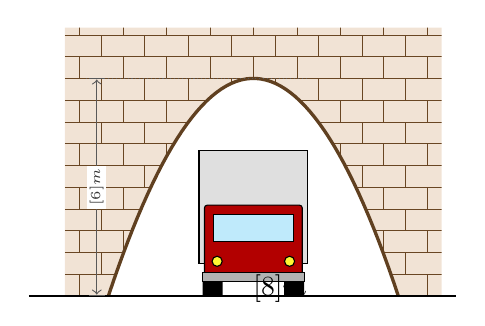
\begin{tikzpicture}[x=0.46cm, y=0.46cm]
	\fill[brown!22, even odd rule] (-5.2,0) rectangle (5.2,7.4) (-4,0) -- plot[domain=-4:4, samples=60] (\x,{-0.375*\x*\x+6}) -- cycle;
	\begin{scope}[even odd rule]
		\clip (-5.2,0) rectangle (5.2,7.4) (-4,0) -- plot[domain=-4:4, samples=60] (\x,{-0.375*\x*\x+6}) -- cycle;
		\foreach \r in {0,...,12} {
			\draw[brown!55!black, very thin] (-5.2,\r*0.6) -- (5.2,\r*0.6);
			\foreach \c in {-5,...,5} \draw[brown!55!black, very thin] ({\c*1.2+0.6*mod(\r,2)},\r*0.6) -- ++(0,0.6);
		}
	\end{scope}
	\draw[very thick, brown!50!black, domain=-4:4, samples=60] plot (\x,{-0.375*\x*\x+6});
	\draw[thick] (-6.2,0) -- (5.6,0);
	%Lkw von vorn
	\fill[black] (-1.4,0) rectangle (-0.85,0.6) (0.85,0) rectangle (1.4,0.6);
	\fill[gray!25, draw=black] (-1.5,0.9) rectangle (1.5,4);
	\fill[red!70!black, draw=black, rounded corners=1pt] (-1.35,0.45) rectangle (1.35,2.5);
	\fill[cyan!25, draw=black] (-1.1,1.5) rectangle (1.1,2.25);
	\fill[gray!60, draw=black] (-1.4,0.4) rectangle (1.4,0.65);
	\fill[yellow!80, draw=black] (-1,0.95) circle (0.14) (1,0.95) circle (0.14);
	\masslinie{(-4,-0.8)}{(4,-0.8)}{$\unit[8]{m}$}
	\draw[thin, black!65, densely dotted] (0,6) -- (-6.1,6);
	\draw[|<->|, thin, black!65] (-5.8,0) -- (-5.8,6) node[midway, fill=white, text=black!80, inner sep=1pt, font=\tiny, rotate=90] {$\unit[6]{m}$};
\end{tikzpicture}
\end{lstlisting}

\begin{ausgabe}
\centering
	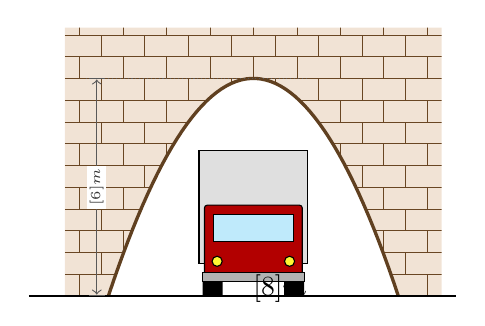
\begin{tikzpicture}[x=0.46cm, y=0.46cm]
		\fill[brown!22, even odd rule] (-5.2,0) rectangle (5.2,7.4) (-4,0) -- plot[domain=-4:4, samples=60] (\x,{-0.375*\x*\x+6}) -- cycle;
		\begin{scope}[even odd rule]
			\clip (-5.2,0) rectangle (5.2,7.4) (-4,0) -- plot[domain=-4:4, samples=60] (\x,{-0.375*\x*\x+6}) -- cycle;
			\foreach \r in {0,...,12} {
				\draw[brown!55!black, very thin] (-5.2,\r*0.6) -- (5.2,\r*0.6);
				\foreach \c in {-5,...,5} \draw[brown!55!black, very thin] ({\c*1.2+0.6*mod(\r,2)},\r*0.6) -- ++(0,0.6);
			}
		\end{scope}
		\draw[very thick, brown!50!black, domain=-4:4, samples=60] plot (\x,{-0.375*\x*\x+6});
		\draw[thick] (-6.2,0) -- (5.6,0);
		%Lkw von vorn
		\fill[black] (-1.4,0) rectangle (-0.85,0.6) (0.85,0) rectangle (1.4,0.6);
		\fill[gray!25, draw=black] (-1.5,0.9) rectangle (1.5,4);
		\fill[red!70!black, draw=black, rounded corners=1pt] (-1.35,0.45) rectangle (1.35,2.5);
		\fill[cyan!25, draw=black] (-1.1,1.5) rectangle (1.1,2.25);
		\fill[gray!60, draw=black] (-1.4,0.4) rectangle (1.4,0.65);
		\fill[yellow!80, draw=black] (-1,0.95) circle (0.14) (1,0.95) circle (0.14);
		\masslinie{(-4,-0.8)}{(4,-0.8)}{$\unit[8]{m}$}
		\draw[thin, black!65, densely dotted] (0,6) -- (-6.1,6);
		\draw[|<->|, thin, black!65] (-5.8,0) -- (-5.8,6) node[midway, fill=white, text=black!80, inner sep=1pt, font=\tiny, rotate=90] {$\unit[6]{m}$};
	\end{tikzpicture}
\end{ausgabe}


%%%%  UNTERKAPITEL  %%%%
\subsection{Brückenbogen mit Schiff}

Der Bogen ist am Wasserspiegel $\unit[20]{m}$ breit und in der Mitte $\unit[5]{m}$ hoch. Ein Schiff ist $\unit[8]{m}$ breit und ragt $\unit[4]{m}$ aus dem Wasser.

\begin{lstlisting}[style=latex]
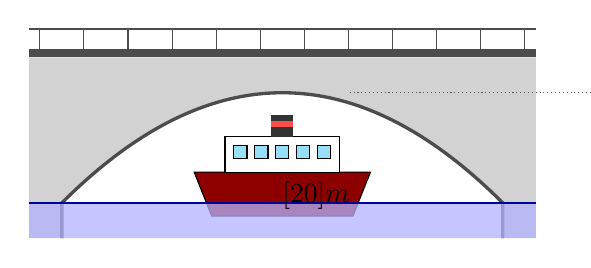
\begin{tikzpicture}[x=0.28cm, y=0.28cm]
	\fill[gray!35, even odd rule] (-11.5,-1.6) rectangle (11.5,6.6) (-10,-1.6) -- (-10,0) -- plot[domain=-10:10, samples=60] (\x,{-0.05*\x*\x+5}) -- (10,-1.6) -- cycle;
	\draw[very thick, gray!60!black] (-10,-1.6) -- (-10,0) -- plot[domain=-10:10, samples=60] (\x,{-0.05*\x*\x+5}) -- (10,-1.6);
	\fill[gray!60!black] (-11.5,6.6) rectangle (11.5,7);
	\foreach \g in {-11,-9,...,11} \draw[gray!60!black] (\g,7) -- (\g,7.9);
	\draw[gray!60!black, thick] (-11.5,7.9) -- (11.5,7.9);
	%Schiff von vorn
	\fill[red!55!black, draw=black] (-4,1.4) -- (4,1.4) -- (3.2,-0.6) -- (-3.2,-0.6) -- cycle;
	\fill[white, draw=black] (-2.6,1.4) rectangle (2.6,3);
	\foreach \f in {-1.9,-0.95,0,0.95,1.9} \fill[cyan!40, draw=black, thin] (\f-0.3,2.0) rectangle (\f+0.3,2.6);
	\fill[black!80] (-0.5,3) rectangle (0.5,4);
	\fill[red!70] (-0.5,3.45) rectangle (0.5,3.7);
	%Wasser
	\fill[blue!30, opacity=0.75] (-11.5,-1.6) rectangle (11.5,0);
	\draw[blue!60!black] (-11.5,0) -- (11.5,0);
	\masslinie{(-10,-2.5)}{(10,-2.5)}{$\unit[20]{m}$}
	\draw[thin, black!65, densely dotted] (0,5) -- (12.6,5) (11.5,0) -- (12.6,0);
	\draw[|<->|, thin, black!65] (12.3,0) -- (12.3,5) node[midway, fill=white, text=black!80, inner sep=1pt, font=\tiny, rotate=90] {$\unit[5]{m}$};
\end{tikzpicture}
\end{lstlisting}

\begin{ausgabe}
\centering
	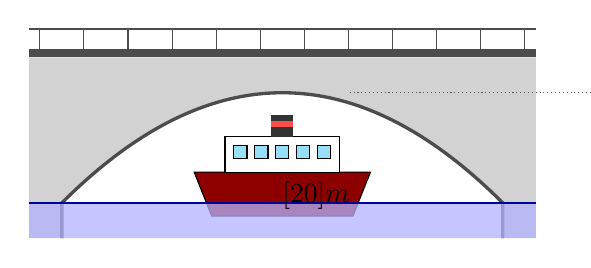
\begin{tikzpicture}[x=0.28cm, y=0.28cm]
		\fill[gray!35, even odd rule] (-11.5,-1.6) rectangle (11.5,6.6) (-10,-1.6) -- (-10,0) -- plot[domain=-10:10, samples=60] (\x,{-0.05*\x*\x+5}) -- (10,-1.6) -- cycle;
		\draw[very thick, gray!60!black] (-10,-1.6) -- (-10,0) -- plot[domain=-10:10, samples=60] (\x,{-0.05*\x*\x+5}) -- (10,-1.6);
		\fill[gray!60!black] (-11.5,6.6) rectangle (11.5,7);
		\foreach \g in {-11,-9,...,11} \draw[gray!60!black] (\g,7) -- (\g,7.9);
		\draw[gray!60!black, thick] (-11.5,7.9) -- (11.5,7.9);
		%Schiff von vorn
		\fill[red!55!black, draw=black] (-4,1.4) -- (4,1.4) -- (3.2,-0.6) -- (-3.2,-0.6) -- cycle;
		\fill[white, draw=black] (-2.6,1.4) rectangle (2.6,3);
		\foreach \f in {-1.9,-0.95,0,0.95,1.9} \fill[cyan!40, draw=black, thin] (\f-0.3,2.0) rectangle (\f+0.3,2.6);
		\fill[black!80] (-0.5,3) rectangle (0.5,4);
		\fill[red!70] (-0.5,3.45) rectangle (0.5,3.7);
		%Wasser
		\fill[blue!30, opacity=0.75] (-11.5,-1.6) rectangle (11.5,0);
		\draw[blue!60!black] (-11.5,0) -- (11.5,0);
		\masslinie{(-10,-2.5)}{(10,-2.5)}{$\unit[20]{m}$}
		\draw[thin, black!65, densely dotted] (0,5) -- (12.6,5) (11.5,0) -- (12.6,0);
		\draw[|<->|, thin, black!65] (12.3,0) -- (12.3,5) node[midway, fill=white, text=black!80, inner sep=1pt, font=\tiny, rotate=90] {$\unit[5]{m}$};
	\end{tikzpicture}
\end{ausgabe}


%%%%  UNTERKAPITEL  %%%%
\subsection{Freistoß}

Der Ball erreicht nach $\unit[10]{m}$ seine größte Höhe von $\unit[3]{m}$. Die Mauer steht bei $\unit[9{,}15]{m}$, das Tor bei $\unit[18]{m}$. Breite Szenen wie diese stehen über die volle Textbreite.

\begin{lstlisting}[style=latex]
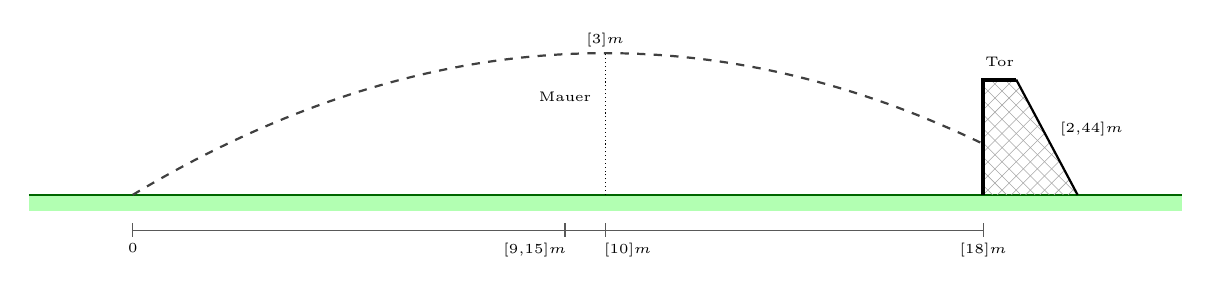
\begin{tikzpicture}[x=0.6cm, y=0.6cm]
	\fill[green!30] (-2.2,-0.35) rectangle (22.2,0);
	\draw[thick, green!40!black] (-2.2,0) -- (22.2,0);
	\emojifigur[xscale=-1]{(-1.1,0)}{person running}{1.08cm}
	\emojifigur{(8.6,0)}{man standing}{1.08cm}
	\emojifigur{(9.15,0)}{woman standing}{1.08cm}
	\emojifigur{(9.7,0)}{person standing}{1.08cm}
	%Tor (Seitenansicht)
	\begin{scope}
		\clip (18,0) -- (18,2.44) -- (18.7,2.44) -- (20,0) -- cycle;
		\foreach \n in {-3,-2.7,...,3} \draw[gray!70, very thin] (18+\n,0) -- ++(2.6,2.6) (20+\n,0) -- ++(-2.6,2.6);
	\end{scope}
	\draw[thick] (18.7,2.44) -- (20,0);
	\draw[line width=1.4pt] (18,0) -- (18,2.44) -- (18.7,2.44);
	\draw[dashed, thick, gray!50!black, domain=0:18, samples=80] plot (\x,{-0.03*(\x-10)^2+3});
	\emojifigur{(0,0)}{soccer ball}{0.27cm}
	\emojifigur{(4.5,1.87)}{soccer ball}{0.27cm}
	\draw[densely dotted, thin] (10,0) -- (10,3) node[above, font=\tiny, inner sep=2pt] {$\unit[3]{m}$};
	\node[font=\tiny, anchor=south, inner sep=1pt] at (9.15,1.9) {Mauer};
	\node[font=\tiny, above] at (18.35,2.5) {Tor};
	\node[font=\tiny, right, inner sep=2pt] at (19.5,1.4) {$\unit[2{,}44]{m}$};
	%Entfernungsleiste
	\draw[thin, black!65] (0,-0.75) -- (18,-0.75);
	\foreach \k in {0,9.15,10,18} \draw[thin, black!65] (\k,-0.6) -- (\k,-0.9);
	\node[font=\tiny, below, inner sep=2pt] at (0,-0.9) {$0$};
	\node[font=\tiny, below left, inner sep=2pt] at (9.3,-0.9) {$\unit[9{,}15]{m}$};
	\node[font=\tiny, below right, inner sep=2pt] at (9.85,-0.9) {$\unit[10]{m}$};
	\node[font=\tiny, below, inner sep=2pt] at (18,-0.9) {$\unit[18]{m}$};
\end{tikzpicture}
\end{lstlisting}

\begin{ausgabe}
\begin{passend}
	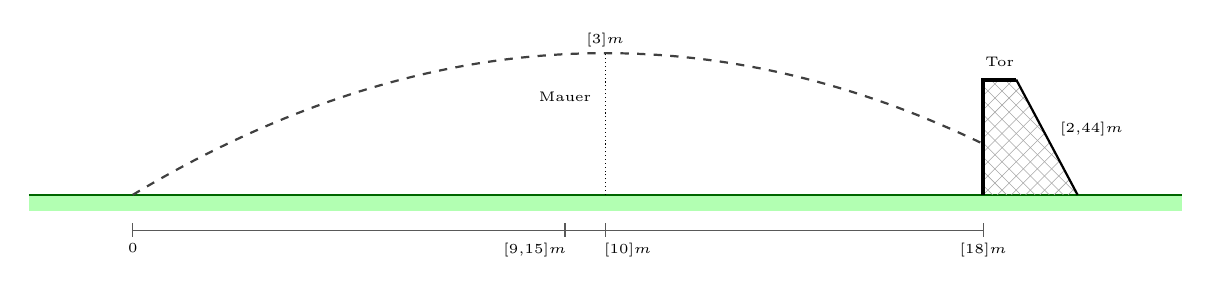
\begin{tikzpicture}[x=0.6cm, y=0.6cm]
		\fill[green!30] (-2.2,-0.35) rectangle (22.2,0);
		\draw[thick, green!40!black] (-2.2,0) -- (22.2,0);
		\emojifigur[xscale=-1]{(-1.1,0)}{person running}{1.08cm}
		\emojifigur{(8.6,0)}{man standing}{1.08cm}
		\emojifigur{(9.15,0)}{woman standing}{1.08cm}
		\emojifigur{(9.7,0)}{person standing}{1.08cm}
		%Tor (Seitenansicht)
		\begin{scope}
			\clip (18,0) -- (18,2.44) -- (18.7,2.44) -- (20,0) -- cycle;
			\foreach \n in {-3,-2.7,...,3} \draw[gray!70, very thin] (18+\n,0) -- ++(2.6,2.6) (20+\n,0) -- ++(-2.6,2.6);
		\end{scope}
		\draw[thick] (18.7,2.44) -- (20,0);
		\draw[line width=1.4pt] (18,0) -- (18,2.44) -- (18.7,2.44);
		\draw[dashed, thick, gray!50!black, domain=0:18, samples=80] plot (\x,{-0.03*(\x-10)^2+3});
		\emojifigur{(0,0)}{soccer ball}{0.27cm}
		\emojifigur{(4.5,1.87)}{soccer ball}{0.27cm}
		\draw[densely dotted, thin] (10,0) -- (10,3) node[above, font=\tiny, inner sep=2pt] {$\unit[3]{m}$};
		\node[font=\tiny, anchor=south, inner sep=1pt] at (9.15,1.9) {Mauer};
		\node[font=\tiny, above] at (18.35,2.5) {Tor};
		\node[font=\tiny, right, inner sep=2pt] at (19.5,1.4) {$\unit[2{,}44]{m}$};
		%Entfernungsleiste
		\draw[thin, black!65] (0,-0.75) -- (18,-0.75);
		\foreach \k in {0,9.15,10,18} \draw[thin, black!65] (\k,-0.6) -- (\k,-0.9);
		\node[font=\tiny, below, inner sep=2pt] at (0,-0.9) {$0$};
		\node[font=\tiny, below left, inner sep=2pt] at (9.3,-0.9) {$\unit[9{,}15]{m}$};
		\node[font=\tiny, below right, inner sep=2pt] at (9.85,-0.9) {$\unit[10]{m}$};
		\node[font=\tiny, below, inner sep=2pt] at (18,-0.9) {$\unit[18]{m}$};
	\end{tikzpicture}
\end{passend}
\end{ausgabe}


%%%%  UNTERKAPITEL  %%%%
\subsection{Leiter an der Hauswand (Satz des Pythagoras)}

Eine $\unit[5]{m}$ lange Leiter steht $\unit[3]{m}$ von der Wand entfernt. Wie hoch reicht sie? Die Sprossen entstehen aus einer Schleife über Zwischenpunkte der Strecke (\texttt{calc}).

\begin{lstlisting}[style=latex]
\begin{tikzpicture}[x=0.7cm, y=0.7cm]
	\fill[green!25] (-3.5,-0.45) rectangle (5,0);
	\draw[thick, green!40!black] (-3.5,0) -- (5,0);
	% Hauswand
	\fill[yellow!25, draw=black] (-3.5,0) rectangle (0,5.4);
	\fill[cyan!30, draw=black] (-2.6,2.6) rectangle (-1.2,4.2);
	% Leiter von (3|0) nach (0|4): zwei Holme, neun Sprossen
	\draw[brown!60!black, line width=3.4pt] (3,0) -- (0,4);
	\draw[white, line width=2pt] (3,0) -- (0,4);
	\foreach \t in {0.1,0.2,...,0.9}
		\draw[brown!60!black, thick] ($(3,0)!\t!(0,4)$) ++(36.87:-1.7pt) -- ++(36.87:3.4pt);
	\emojifigur{(4.1,0)}{person standing}{1.26cm}
	% rechter Winkel und Beschriftung
	\draw[thin] (0,0.4) -- (0.4,0.4) -- (0.4,0);
	\node[font=\scriptsize, above right, inner sep=2pt] at (1.5,2) {$\unit[5]{m}$};
	\masslinie{(0,-0.8)}{(3,-0.8)}{$\unit[3]{m}$}
	\node[font=\scriptsize, left, inner sep=3pt, fill=yellow!25] at (0,2) {$h$};
\end{tikzpicture}
\end{lstlisting}

\begin{ausgabe}
\centering
	\begin{tikzpicture}[x=0.7cm, y=0.7cm]
		\fill[green!25] (-3.5,-0.45) rectangle (5,0);
		\draw[thick, green!40!black] (-3.5,0) -- (5,0);
		% Hauswand
		\fill[yellow!25, draw=black] (-3.5,0) rectangle (0,5.4);
		\fill[cyan!30, draw=black] (-2.6,2.6) rectangle (-1.2,4.2);
		% Leiter von (3|0) nach (0|4): zwei Holme, neun Sprossen
		\draw[brown!60!black, line width=3.4pt] (3,0) -- (0,4);
		\draw[white, line width=2pt] (3,0) -- (0,4);
		\foreach \t in {0.1,0.2,...,0.9}
			\draw[brown!60!black, thick] ($(3,0)!\t!(0,4)$) ++(36.87:-1.7pt) -- ++(36.87:3.4pt);
		\emojifigur{(4.1,0)}{person standing}{1.26cm}
		% rechter Winkel und Beschriftung
		\draw[thin] (0,0.4) -- (0.4,0.4) -- (0.4,0);
		\node[font=\scriptsize, above right, inner sep=2pt] at (1.5,2) {$\unit[5]{m}$};
		\masslinie{(0,-0.8)}{(3,-0.8)}{$\unit[3]{m}$}
		\node[font=\scriptsize, left, inner sep=3pt, fill=yellow!25] at (0,2) {$h$};
	\end{tikzpicture}
\end{ausgabe}


%%%%  UNTERKAPITEL  %%%%
\subsection{Schattenwurf (Strahlensatz)}

Ein $\unit[1{,}50]{m}$ langer Stab wirft einen $\unit[2]{m}$ langen Schatten, der Baum einen $\unit[12]{m}$ langen. Wie hoch ist der Baum? Der Sonnenstrahl ist eine einzige Strecke von der Baumspitze zur Schattenspitze. Der Stab steht so, dass seine Spitze genau auf dem Strahl liegt.

\begin{lstlisting}[style=latex]
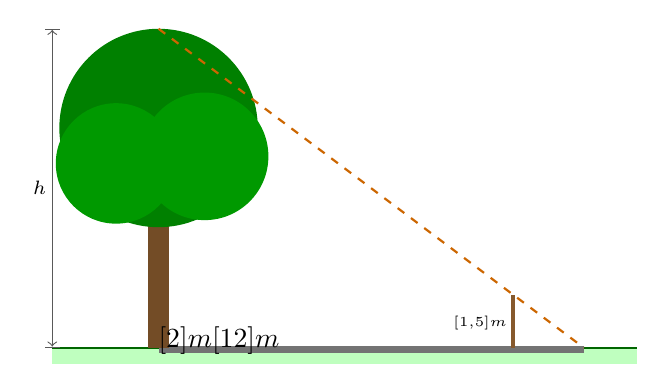
\begin{tikzpicture}[x=0.45cm, y=0.45cm]
	\fill[green!25] (-3,-0.45) rectangle (13.5,0);
	\draw[thick, green!40!black] (-3,0) -- (13.5,0);
	% Schatten
	\draw[black!55, line width=2.5pt] (0,-0.05) -- (12,-0.05);
	% Baum: 9 m hoch
	\fill[brown!60!black] (-0.3,0) rectangle (0.3,4);
	\fill[green!50!black] (0,6.2) circle (2.8);
	\fill[green!60!black] (-1.2,5.2) circle (1.7) (1.3,5.4) circle (1.8);
	% Sonnenstrahl und Stab (1,5 m hoch, 2 m vor der Schattenspitze)
	\draw[orange!80!black, thick, dashed] (0,9) -- (12,0);
	\draw[very thick, brown!70!black] (10,0) -- (10,1.5);
	\emojifigur{(-2,7.6)}{sun}{0.9cm}
	\node[font=\scriptsize, left, inner sep=2pt] at (-3,4.5) {$h$};
	\draw[thin, black!65, |<->|] (-3,0) -- (-3,9);
	\node[font=\tiny, left, inner sep=2pt] at (10,0.7) {$\unit[1{,}5]{m}$};
	\masslinie{(10,-0.9)}{(12,-0.9)}{$\unit[2]{m}$}
	\masslinie{(0,-1.8)}{(12,-1.8)}{$\unit[12]{m}$}
\end{tikzpicture}
\end{lstlisting}

\begin{ausgabe}
\centering
	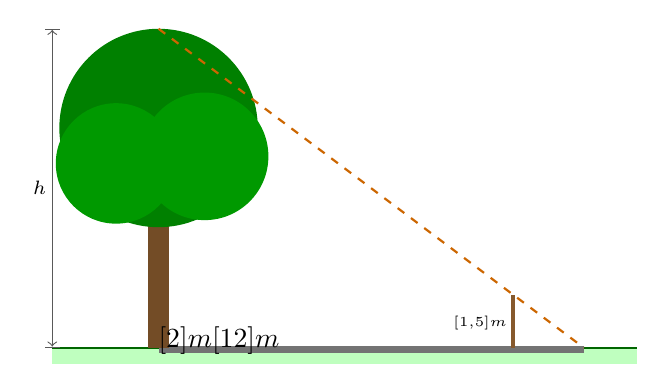
\begin{tikzpicture}[x=0.45cm, y=0.45cm]
		\fill[green!25] (-3,-0.45) rectangle (13.5,0);
		\draw[thick, green!40!black] (-3,0) -- (13.5,0);
		% Schatten
		\draw[black!55, line width=2.5pt] (0,-0.05) -- (12,-0.05);
		% Baum: 9 m hoch
		\fill[brown!60!black] (-0.3,0) rectangle (0.3,4);
		\fill[green!50!black] (0,6.2) circle (2.8);
		\fill[green!60!black] (-1.2,5.2) circle (1.7) (1.3,5.4) circle (1.8);
		% Sonnenstrahl und Stab (1,5 m hoch, 2 m vor der Schattenspitze)
		\draw[orange!80!black, thick, dashed] (0,9) -- (12,0);
		\draw[very thick, brown!70!black] (10,0) -- (10,1.5);
		\emojifigur{(-2,7.6)}{sun}{0.9cm}
		\node[font=\scriptsize, left, inner sep=2pt] at (-3,4.5) {$h$};
		\draw[thin, black!65, |<->|] (-3,0) -- (-3,9);
		\node[font=\tiny, left, inner sep=2pt] at (10,0.7) {$\unit[1{,}5]{m}$};
		\masslinie{(10,-0.9)}{(12,-0.9)}{$\unit[2]{m}$}
		\masslinie{(0,-1.8)}{(12,-1.8)}{$\unit[12]{m}$}
	\end{tikzpicture}
\end{ausgabe}


%%%%  UNTERKAPITEL  %%%%
\subsection{Straße mit Steigung}

Eine Straße steigt auf $\unit[100]{m}$ waagerechter Strecke um $\unit[12]{m}$. Das Auto wird um den Steigungswinkel gedreht und auf die Fahrbahn gesetzt.

\begin{lstlisting}[style=latex]
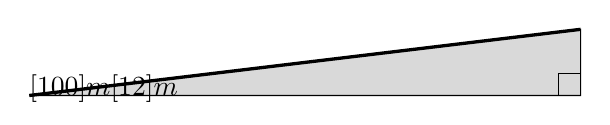
\begin{tikzpicture}[x=0.07cm, y=0.07cm]   % 1 m entspricht 0,07 cm
	\fill[gray!30, draw=black] (0,0) -- (100,0) -- (100,12) -- cycle;
	\draw[very thick] (0,0) -- (100,12);
	\emojifigur[rotate=6.84]{(45,5.4)}{automobile}{0.8cm}
	\draw[thin] (96,0) -- (96,4) -- (100,4);
	\masslinie{(0,-6)}{(100,-6)}{$\unit[100]{m}$}
	\masslinie{(106,0)}{(106,12)}{$\unit[12]{m}$}
\end{tikzpicture}
\end{lstlisting}

\begin{ausgabe}
\begin{passend}
	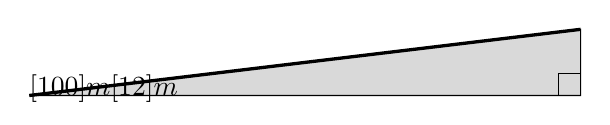
\begin{tikzpicture}[x=0.07cm, y=0.07cm]   % 1 m entspricht 0,07 cm
		\fill[gray!30, draw=black] (0,0) -- (100,0) -- (100,12) -- cycle;
		\draw[very thick] (0,0) -- (100,12);
		\emojifigur[rotate=6.84]{(45,5.4)}{automobile}{0.8cm}
		\draw[thin] (96,0) -- (96,4) -- (100,4);
		\masslinie{(0,-6)}{(100,-6)}{$\unit[100]{m}$}
		\masslinie{(106,0)}{(106,12)}{$\unit[12]{m}$}
	\end{tikzpicture}
\end{passend}
\end{ausgabe}



%%%%  KAPITEL  %%%%
\section{Das Lösungsbild: ein Koordinatensystem hinter der Skizze}\label{sec:loesungsbild}

Weil die Skizze in Metern gezeichnet ist, passt ein Koordinatensystem ohne Umrechnen darunter. Im Lösungsteil sieht man dann, dass der Wasserstrahl, das Seil oder der Bogen wirklich der Graph der Funktion ist, und kann Scheitelpunkt, Nullstellen und berechnete Punkte ablesen.


%%%%  UNTERKAPITEL  %%%%
\subsection{Raster und markante Punkte}

\texttt{\textbackslash skizzenraster} zeichnet ein feines Gitter, beide Achsen und die Beschriftungen, die in den beiden Listen stehen. Der Befehl kommt \emph{vor} den Gegenständen, damit das Raster dahinter liegt. \texttt{\textbackslash skizzenpunkt} markiert einen Punkt und beschriftet ihn auf halb durchsichtigem weißem Grund. Der Graph selbst wird in der Akzentfarbe durchgezogen.

\begin{lstlisting}[style=latex]
\begin{tikzpicture}[x=0.5cm, y=0.5cm]
	\skizzenraster{-1}{11}{0}{4}{1}{2,4,6,8,10}{1,2,3,4}
	\draw[thick, orange!50!black] (-2,0) -- (11.2,0);
	\emojifigur[xscale=-1]{(-0.85,0)}{person playing handball}{1.25cm}
	\draw[akzentblau, thick, domain=0:10, samples=100] plot (\x,{-0.1*(\x-4)^2+3.6});
	\skizzenpunkt{(0,2)}{above left}{$(0\,|\,2)$}
	\skizzenpunkt{(4,3.6)}{above}{$S(4\,|\,3{,}6)$}
	\skizzenpunkt{(10,0)}{above right}{$N(10\,|\,0)$}
\end{tikzpicture}
\end{lstlisting}

\begin{ausgabe}
\centering
	\begin{tikzpicture}[x=0.5cm, y=0.5cm]
		\skizzenraster{-1}{11}{0}{4}{1}{2,4,6,8,10}{1,2,3,4}
		\draw[thick, orange!50!black] (-2,0) -- (11.2,0);
		\emojifigur[xscale=-1]{(-0.85,0)}{person playing handball}{1.25cm}
		\draw[akzentblau, thick, domain=0:10, samples=100] plot (\x,{-0.1*(\x-4)^2+3.6});
		\skizzenpunkt{(0,2)}{above left}{$(0\,|\,2)$}
		\skizzenpunkt{(4,3.6)}{above}{$S(4\,|\,3{,}6)$}
		\skizzenpunkt{(10,0)}{above right}{$N(10\,|\,0)$}
	\end{tikzpicture}
\end{ausgabe}

Liegt eine gefüllte Fläche (Mauer, Brücke) im Weg, wird sie im Lösungsbild mit \texttt{\textbackslash fill[white, opacity=0.55]} aufgehellt und das Raster danach gezeichnet.


%%%%  UNTERKAPITEL  %%%%
\subsection{Ein Bild, zwei Fassungen}

Aufgabenbild und Lösungsbild sollen dasselbe Bild sein. Deshalb wird die Skizze einmal als Befehl definiert. Der Schalter \texttt{\textbackslash ifmitKS} entscheidet, was gezeichnet wird: im Aufgabenteil Untergrund und Maße, im Lösungsteil Raster und markante Punkte. Aufgerufen wird die Skizze mit \texttt{\textbackslash skizzeSpringbrunnen}, das Lösungsbild mit \texttt{\{\textbackslash mitKStrue \textbackslash skizzeSpringbrunnen\}}. Die geschweiften Klammern sorgen dafür, dass der Schalter danach wieder aus ist.

\begin{lstlisting}[style=latex]
\newcommand{\skizzeSpringbrunnen}{%
\begin{tikzpicture}[x=0.5cm, y=0.5cm]
	\ifmitKS \skizzenraster{0}{11}{0}{6}{1}{2,4,6,8,10}{1,2,3,4,5}
	\else \fill[green!25] (-1.2,-0.45) rectangle (11.2,0); \fill[gray!60] (-0.7,-0.45) rectangle (0.7,0); \fi
	\draw[thick, green!40!black] (-1.2,0) -- (11.2,0);
	\fill[gray!80!black] (-0.12,0) rectangle (0.12,0.3);
	\draw[blue!35, line width=3pt, line cap=round, domain=0:10, samples=100] plot (\x,{-0.2*(\x-5)^2+5});
	\draw[blue!75, line width=1.1pt, line cap=round, domain=0:10, samples=100] plot (\x,{-0.2*(\x-5)^2+5});
	\foreach \a in {25,55,90,125,155} \draw[blue!70, thin] (10,0.05) -- ++(\a:0.45);
	\emojifigur{(8.5,0)}{man standing}{0.9cm}
	\ifmitKS
		\draw[densely dashed, red] (8.5,1.8) -- (8.5,2.55);
		\skizzenpunkt{(5,5)}{above}{$S(5\,|\,5)$}
		\skizzenpunkt{(10,0)}{above right}{$N(10\,|\,0)$}
		\skizzenpunkt{(8.5,2.55)}{right=2pt}{$(8{,}5\,|\,2{,}55)$}
	\else
		\node[font=\tiny, above left] at (-0.1,0.15) {Düse};
		\masslinie{(0,-1.1)}{(8.5,-1.1)}{$\unit[8{,}5]{m}$}
		\node[font=\tiny, left, inner sep=2pt] at (8.05,0.9) {$\unit[1{,}80]{m}$};
	\fi
\end{tikzpicture}}

% Aufgabenbild und Lösungsbild
\skizzeSpringbrunnen \hfill {\mitKStrue \skizzeSpringbrunnen}
\end{lstlisting}

\newcommand{\skizzeSpringbrunnen}{%
\begin{tikzpicture}[x=0.5cm, y=0.5cm]
	\ifmitKS \skizzenraster{0}{11}{0}{6}{1}{2,4,6,8,10}{1,2,3,4,5}
	\else \fill[green!25] (-1.2,-0.45) rectangle (11.2,0); \fill[gray!60] (-0.7,-0.45) rectangle (0.7,0); \fi
	\draw[thick, green!40!black] (-1.2,0) -- (11.2,0);
	\fill[gray!80!black] (-0.12,0) rectangle (0.12,0.3);
	\draw[blue!35, line width=3pt, line cap=round, domain=0:10, samples=100] plot (\x,{-0.2*(\x-5)^2+5});
	\draw[blue!75, line width=1.1pt, line cap=round, domain=0:10, samples=100] plot (\x,{-0.2*(\x-5)^2+5});
	\foreach \a in {25,55,90,125,155} \draw[blue!70, thin] (10,0.05) -- ++(\a:0.45);
	\emojifigur{(8.5,0)}{man standing}{0.9cm}
	\ifmitKS
		\draw[densely dashed, red] (8.5,1.8) -- (8.5,2.55);
		\skizzenpunkt{(5,5)}{above}{$S(5\,|\,5)$}
		\skizzenpunkt{(10,0)}{above right}{$N(10\,|\,0)$}
		\skizzenpunkt{(8.5,2.55)}{right=2pt}{$(8{,}5\,|\,2{,}55)$}
	\else
		\node[font=\tiny, above left] at (-0.1,0.15) {Düse};
		\masslinie{(0,-1.1)}{(8.5,-1.1)}{$\unit[8{,}5]{m}$}
		\node[font=\tiny, left, inner sep=2pt] at (8.05,0.9) {$\unit[1{,}80]{m}$};
	\fi
\end{tikzpicture}}

\begin{ausgabe}
	\skizzeSpringbrunnen \hfill {\mitKStrue \skizzeSpringbrunnen}
\end{ausgabe}

Ein solcher Skizzen-Befehl gehört zu einem einzelnen Arbeitsblatt und steht deshalb in dessen Präambel, nicht in der \texttt{newcommands.tex}.



%%%%  KAPITEL  %%%%
\section{Dialoge und Fehlersuche}

Fehlersuchaufgaben werden lebendiger, wenn nicht eine Liste, sondern Personen etwas behaupten. Die Lernenden prüfen dann Aussagen und nicht Stichpunkte.


%%%%  UNTERKAPITEL  %%%%
\subsection{Mehrere Köpfe mit Sprechblasen}

\texttt{\textbackslash emojisprecher} setzt einen Emoji-Kopf an die Stelle $x$, einen Namen darunter und eine Sprechblase darüber. Alle Blasen sind gleich breit und wachsen nach oben. Die Nummer in der Blase verbindet Aufgabe und Lösung.

\begin{lstlisting}[style=latex]
\begin{tikzpicture}
	\emojisprecher{0}{boy}{A}{\textbf{(i)} Der Scheitelpunkt ist $S(3\,|\,1)$.}
	\emojisprecher{2.8}{girl: medium skin tone}{B}{\textbf{(ii)} Der Graph ist nach oben geöffnet.}
	\emojisprecher{5.6}{boy: medium-dark skin tone}{C}{\textbf{(iii)} Der Graph ist gestreckt.}
	\emojisprecher{8.4}{girl: dark skin tone}{D}{\textbf{(iv)} Der Wertebereich ist $1\le y<\infty$.}
\end{tikzpicture}
\end{lstlisting}

\begin{ausgabe}
\centering
	\begin{tikzpicture}
		\emojisprecher{0}{boy}{A}{\textbf{(i)} Der Scheitelpunkt ist $S(3\,|\,1)$.}
		\emojisprecher{2.8}{girl: medium skin tone}{B}{\textbf{(ii)} Der Graph ist nach oben geöffnet.}
		\emojisprecher{5.6}{boy: medium-dark skin tone}{C}{\textbf{(iii)} Der Graph ist gestreckt.}
		\emojisprecher{8.4}{girl: dark skin tone}{D}{\textbf{(iv)} Der Wertebereich ist $1\le y<\infty$.}
	\end{tikzpicture}
\end{ausgabe}


%%%%  UNTERKAPITEL  %%%%
\subsection{Zwei im Gespräch}

Für ein Gespräch stehen die Köpfe links und rechts, die Blasen dazwischen. Jede Blase bekommt einen kurzen Zipfel zur eigenen Seite: Bei den linken Blasen ist der Anker \texttt{west}, der Zipfel zeigt nach links, bei den rechten umgekehrt.

\begin{lstlisting}[style=latex]
\begin{tikzpicture}[blase/.style={rectangle callout, rounded corners=2pt, draw, fill=white,
                                  font=\scriptsize, inner sep=3pt}]
	\node[inner sep=0pt] at (0,0)  {\twemoji[height=1.2cm]{boy: medium skin tone}};
	\node[inner sep=0pt] at (12,0) {\twemoji[height=1.2cm]{girl}};
	\node[blase, anchor=west, callout absolute pointer={(0.85,0.68)}] at (1.25,0.8)
		{\textbf{(i)} Der Scheitelpunkt ist $S(4\,|\,{-2})$.};
	\node[blase, anchor=east, callout absolute pointer={(11.15,0.08)}] at (10.75,0.2)
		{\textbf{(ii)} Dann ist der Graph gestreckt.};
	\node[blase, anchor=west, callout absolute pointer={(0.85,-0.52)}] at (1.25,-0.4)
		{\textbf{(iii)} Die Funktion hat keine Nullstellen.};
\end{tikzpicture}
\end{lstlisting}

\begin{ausgabe}
\begin{passend}
	\begin{tikzpicture}[blase/.style={rectangle callout, rounded corners=2pt, draw, fill=white,
	                                  font=\scriptsize, inner sep=3pt}]
		\node[inner sep=0pt] at (0,0)  {\twemoji[height=1.2cm]{boy: medium skin tone}};
		\node[inner sep=0pt] at (12,0) {\twemoji[height=1.2cm]{girl}};
		\node[blase, anchor=west, callout absolute pointer={(0.85,0.68)}] at (1.25,0.8)
			{\textbf{(i)} Der Scheitelpunkt ist $S(4\,|\,{-2})$.};
		\node[blase, anchor=east, callout absolute pointer={(11.15,0.08)}] at (10.75,0.2)
			{\textbf{(ii)} Dann ist der Graph gestreckt.};
		\node[blase, anchor=west, callout absolute pointer={(0.85,-0.52)}] at (1.25,-0.4)
			{\textbf{(iii)} Die Funktion hat keine Nullstellen.};
	\end{tikzpicture}
\end{passend}
\end{ausgabe}


%%%%  UNTERKAPITEL  %%%%
\subsection{Ein Notizzettel mit einer Rechnung}

Eine fehlerhafte Rechnung wirkt wie aus dem Heft, wenn sie auf einem leicht gedrehten gelben Zettel mit Schatten steht (\texttt{drop shadow} aus der Bibliothek \texttt{shadows}). Daneben kommentiert die Person ihr Ergebnis.

\begin{lstlisting}[style=latex]
\begin{tikzpicture}
	\node[draw=gray, fill=yellow!25, drop shadow, rotate=-2, inner sep=6pt, align=left, font=\footnotesize] (z)
		{$f(x)=a(x-2)^2+3$\\[1pt] $-5=a\cdot(0-2)^2+3$\\[1pt] $-5=4a+3$\\[1pt]
		 $\phantom{-5}\,a=-2$\\[1pt] $\underline{\underline{f(x)=-2(x-2)^2+3}}$};
	\node[inner sep=0pt, anchor=south west] (e) at ($(z.south east)+(0.5,0)$)
		{\twemoji[height=1.15cm]{girl: medium-light skin tone}};
	\node[rectangle callout, rounded corners=2pt, draw, fill=white, font=\scriptsize, align=center,
	      anchor=south, inner sep=3pt, callout absolute pointer={($(e.north)+(0,0.05)$)}]
		at ($(e.north)+(0.2,0.45)$) {Probe mit $P$:\\ $f(0)=-5$ \;\ding{52}};
\end{tikzpicture}
\end{lstlisting}

\begin{ausgabe}
\centering
	\begin{tikzpicture}
		\node[draw=gray, fill=yellow!25, drop shadow, rotate=-2, inner sep=6pt, align=left, font=\footnotesize] (z)
			{$f(x)=a(x-2)^2+3$\\[1pt] $-5=a\cdot(0-2)^2+3$\\[1pt] $-5=4a+3$\\[1pt]
			 $\phantom{-5}\,a=-2$\\[1pt] $\underline{\underline{f(x)=-2(x-2)^2+3}}$};
		\node[inner sep=0pt, anchor=south west] (e) at ($(z.south east)+(0.5,0)$)
			{\twemoji[height=1.15cm]{girl: medium-light skin tone}};
		\node[rectangle callout, rounded corners=2pt, draw, fill=white, font=\scriptsize, align=center,
		      anchor=south, inner sep=3pt, callout absolute pointer={($(e.north)+(0,0.05)$)}]
			at ($(e.north)+(0.2,0.45)$) {Probe mit $P$:\\ $f(0)=-5$ \;\ding{52}};
	\end{tikzpicture}
\end{ausgabe}



%%%%  KAPITEL  %%%%
\section{Einbau ins Arbeitsblatt}


%%%%  UNTERKAPITEL  %%%%
\subsection{Skizze neben dem Aufgabentext}

Text und Bild stehen in zwei \texttt{minipage}-Umgebungen nebeneinander, beide oben ausgerichtet. \texttt{\textbackslash vspace\{0pt\}} am Anfang der rechten Spalte sorgt dafür, dass die Oberkante des Bildes auf Höhe der ersten Textzeile liegt. Für die Textspalte haben sich $56$ bis $62\,\%$ der Zeilenbreite bewährt.

\begin{lstlisting}[style=latex]
\begin{enumerate}[(1)]
	\item
		\begin{minipage}[t]{0.58\linewidth}
			Der Wasserstrahl eines Springbrunnens lässt sich durch die Funktion $h$ mit
			$h(x)=-0{,}2(x-5)^2+5$ beschreiben.
			\begin{enumerate}[(a)]
				\item Gib die maximale Höhe des Wasserstrahls an.
				\item Berechne, in welcher Entfernung von der Düse der Strahl auftrifft.
			\end{enumerate}
		\end{minipage}\hfill
		\begin{minipage}[t]{0.40\linewidth}
			\vspace{0pt}\centering
			\skizzeSpringbrunnen
		\end{minipage}
\end{enumerate}
\end{lstlisting}

\begin{ausgabe}
	\begin{enumerate}[(1)]
		\item
			\begin{minipage}[t]{0.58\linewidth}
				Der Wasserstrahl eines Springbrunnens lässt sich durch die Funktion $h$ mit
				$h(x)=-0{,}2(x-5)^2+5$ beschreiben.
				\begin{enumerate}[(a)]
					\item Gib die maximale Höhe des Wasserstrahls an.
					\item Berechne, in welcher Entfernung von der Düse der Strahl auftrifft.
				\end{enumerate}
			\end{minipage}\hfill
			\begin{minipage}[t]{0.40\linewidth}
				\vspace{0pt}\centering
				\skizzeSpringbrunnen
			\end{minipage}
	\end{enumerate}
\end{ausgabe}


%%%%  UNTERKAPITEL  %%%%
\subsection{Breite Bilder und der Lösungsteil}

Eine breite Szene wie der Freistoß steht zentriert zwischen Aufgabentext und Teilaufgaben. Die Umgebung \texttt{passend} aus der \texttt{newcommands.tex} verkleinert ein Bild nur dann, wenn es breiter als die Zeile ist.

Im Lösungsteil steht das Lösungsbild rechts neben der Rechnung. Weil der Lösungsteil in \texttt{scriptsize} gesetzt ist, wird das Bild mit \texttt{\textbackslash resizebox\{\textbackslash linewidth\}\{!\}\{...\}} auf die Spaltenbreite gebracht:

\begin{lstlisting}[style=latex]
\begin{minipage}[t]{0.60\linewidth}
	\vspace{0pt}\raggedright
	... Rechnung ...
\end{minipage}\hfill
\begin{minipage}[t]{0.38\linewidth}
	\vspace{0pt}\centering
	\resizebox{\linewidth}{!}{{\mitKStrue \skizzeSpringbrunnen}}
\end{minipage}
\end{lstlisting}



%%%%  KAPITEL  %%%%
\section{Stolpersteine}

\begin{itemize}
	\item \textbf{Negative Werte potenzieren:} In \texttt{plot} immer \texttt{(\textbackslash x-4)\textasciicircum 2} oder \texttt{\textbackslash x*\textbackslash x} schreiben. \texttt{-\textbackslash x\textasciicircum 2} ohne Klammern rechnet pgf anders als erwartet.
	\item \textbf{\texttt{even odd rule} beim Ausschneiden:} Die Option gehört an \texttt{\textbackslash fill} bzw. an die \texttt{scope}. \texttt{\textbackslash clip[even odd rule]} meldet einen Fehler, weil \texttt{\textbackslash clip} keine Optionen annimmt.
	\item \textbf{Ein \texttt{\textbackslash clip} vergrößert das Bild:} Reicht der Ausschnitt weit über die Zeichnung hinaus, entsteht darunter oder darüber eine Lücke auf dem Blatt. Den Ausschnitt deshalb knapp wählen.
	\item \textbf{Muster:} \texttt{pattern=bricks} und \texttt{pattern=crosshatch} zeigt nicht jeder PDF-Betrachter. Fugen und Netze aus einer Schleife zeichnen.
	\item \textbf{tikzpeople-Figuren sind Büsten.} Für maßstäbliche Personen \texttt{\textbackslash emojifigur} oder das Piktogramm verwenden.
	\item \textbf{Emojis sind farbig.} Im Schwarz-Weiß-Druck bleiben sie erkennbar, wirken aber flauer. Wer nur schwarz-weiß druckt, nimmt das Piktogramm.
	\item \textbf{Die Skizze verrät nichts:} Vor dem Drucken prüfen, ob im Aufgabenbild Zahlen stehen, die erst berechnet werden sollen.
\end{itemize}



%%%%  KAPITEL  %%%%
\section{Zusammenfassung}

\begin{itemize}
	\item Maßstab in die Optionen schreiben (\texttt{x=0.5cm, y=0.5cm}) und in Metern zeichnen.
	\item Reihenfolge: Untergrund, Gegenstände und Figuren, Kurve, Beschriftung.
	\item Figuren mit \texttt{\textbackslash emojifigur} maßstäblich auf den Boden stellen, Hauttöne mischen.
	\item Kurven mit \texttt{plot} aus der Funktionsgleichung zeichnen, Punkte auf der Kurve von Ti\textit{k}Z berechnen lassen.
	\item Höchstens zwei bis drei dezente Maße, sonst eine Entfernungsleiste.
	\item Gegenstände von vorn aus Rechtecken bauen, Umriss exakt nach den Maßen der Aufgabe.
	\item Skizze als Befehl definieren und mit \texttt{\textbackslash ifmitKS} ein Lösungsbild mit Koordinatensystem erzeugen.
	\item Fehlersuche als Gespräch: \texttt{\textbackslash emojisprecher} oder Blasen links und rechts.
\end{itemize}

Mit diesen Bausteinen entsteht eine neue Skizze in wenigen Minuten: eine der neun Vorlagen kopieren, Maßstab und Funktionsgleichung anpassen, Figur und Gegenstand austauschen.

\end{document}
